\documentclass[11pt,a4paper]{article}
\usepackage[margin=24mm,headheight=15pt]{geometry}
\usepackage[T1]{fontenc}
\usepackage{lmodern}
\usepackage{graphicx}
\usepackage{booktabs,tabularx,longtable,array}
\usepackage{amsmath}
\usepackage{xcolor}
\usepackage{listings}
\usepackage{float}
\usepackage{fancyhdr}
\usepackage{hyperref}
\definecolor{accent}{HTML}{17566A}
\definecolor{codebg}{HTML}{F3F6F8}
\hypersetup{colorlinks=true,linkcolor=accent,urlcolor=accent,citecolor=accent,
  pdftitle={Rate-Limited Sender Functionality in picoquic},
  pdfauthor={Aryan Bokolia; Affan Arshad; Soumyadeep Raj; Kevin Shiju George; Aryan Sanjay palimkar}}
\pagestyle{fancy}
\fancyhf{}
\fancyhead[L]{\small Project 16: Rate-Limited CUBIC}
\fancyhead[R]{\small Final project report}
\fancyfoot[C]{\thepage}
\setlength{\parindent}{0pt}
\setlength{\parskip}{6pt}
\setlength{\emergencystretch}{2em}
\renewcommand{\arraystretch}{1.15}
\lstset{basicstyle=\ttfamily\footnotesize,backgroundcolor=\color{codebg},
  frame=single,rulecolor=\color{black!12},breaklines=true,columns=fullflexible,
  keepspaces=true,showstringspaces=false,xleftmargin=3pt,xrightmargin=3pt}
\newcommand{\code}[1]{\texttt{\detokenize{#1}}}
% Generated exclusively from the fresh logs by analyze_results.py.
\newcommand{\BaselineCommit}{5a4eba475555}
\newcommand{\ImplementationCommit}{60323926df8e}
\newcommand{\WindowChange}{98.71}
\newcommand{\BulkChange}{1.23}
\newcommand{\ObservedRateFlight}{3426}
\newcommand{\RateBaselineThroughput}{0.190}
\newcommand{\RateBaselineCwnd}{15.000}
\newcommand{\RateRliThroughput}{0.190}
\newcommand{\RateRliCwnd}{29.806}
\newcommand{\BulkBaselineThroughput}{17.732}
\newcommand{\BulkBaselineCwnd}{213.424}
\newcommand{\BulkRliThroughput}{17.950}
\newcommand{\BulkRliCwnd}{234.478}
\newcommand{\TestCountSummary}{baseline: 562 + 105 subtests; rli: 563 + 105 subtests}


\begin{document}
\hypersetup{pageanchor=false}
\begin{titlepage}
\centering
\vspace*{10mm}
{\Large\color{accent} PROJECT REPORT}\par
\vspace{7mm}
{\large Project \#16}\par
\vspace{10mm}
{\Huge\bfseries Implementation of\\[3mm] Rate-Limited Sender\\[3mm] Functionality in picoquic}\par
\vspace{8mm}
{\Large CUBIC congestion control: baseline, implementation,\\ verification, and experimental evaluation}\par
\vspace{10mm}
\rule{0.8\textwidth}{0.7pt}\par
\vspace{7mm}
{\large Team members}\par
\vspace{3mm}
{\Large\bfseries Aryan Bokolia\\[2mm]
Affan Arshad\\[2mm]
Soumyadeep Raj\\[2mm]
Kevin Shiju George\\[2mm]
Aryan Sanjay palimkar}\par
\vspace{7mm}
{\large 7 November 2026}\par
\vspace{6mm}
{\normalsize Baseline revision: \texttt{\BaselineCommit}\\
Evaluated implementation: \texttt{\ImplementationCommit}}\par
\vfill
\begin{minipage}{0.85\textwidth}
\small Implementation and experimental evaluation of bounded congestion-window
growth for application-limited QUIC connections.
\end{minipage}
\end{titlepage}
\pagenumbering{roman}
\hypersetup{pageanchor=true}

\section*{Abstract}
\addcontentsline{toc}{section}{Abstract}
This project adds an optional Rate-Limited Increase (RLI) mode to CUBIC in
picoquic. The existing CUBIC implementation suppresses window growth when
the sender lacks enough application data to fill its congestion window. The
new mode permits acknowledgement-driven growth while bounding it using a
per-path flight-size history. It implements initialization and reset rules,
Slow Start and congestion-avoidance limits, recovery handling, and qlog
instrumentation, with an explicit runtime switch for comparison.

The unchanged baseline was rebuilt from commit \texttt{\BaselineCommit};
the implementation was built from \texttt{\ImplementationCommit}. Both
passed their complete registered CTest suites on Linux, and the focused
\code{cubic_rli} test passed. Twelve single-flow network-namespace experiments
cover two workloads, two versions, and three repetitions per combination.
For the rate-limited stream, the mean time-weighted cwnd changed by
\WindowChange\%, while the final window rose from 15 KiB to 30 KiB.
The application still supplies approximately 192 kbit/s, so this does not
imply a doubling of throughput. Mean bulk throughput was
\BulkBaselineThroughput{} Mbit/s for baseline and
\BulkRliThroughput{} Mbit/s for RLI, a \BulkChange\% difference.
Six additional experiments run two bulk flows concurrently over a full
dumbbell topology. The results demonstrate bounded window growth and
characterize the implementation under both isolated and competing traffic.

\tableofcontents
\clearpage
\pagenumbering{arabic}

\section{Project details and objectives}
The assignment is to implement rate-limited sender functionality in picoquic,
using CUBIC as the congestion control algorithm and Linux network namespaces
as the experiment environment. The reference is the IETF CCWG work in
progress, \emph{Increase of the Congestion Window when the Sender Is
Rate-Limited}, revision 11 \cite{rli}.

The engineering objectives are to identify how baseline CUBIC handles a
sender with insufficient data, implement bounded growth, preserve ordinary
congestion responses and opt-out behavior, log the necessary state, and
compare observed traces against the intended rules. The report includes
the code locations, test evidence, experiment workflow, results, and known
limits of the conclusions.

\begin{longtable}{p{0.07\textwidth}p{0.37\textwidth}p{0.48\textwidth}}
\toprule Step & Assignment requirement & Evidence in this project\\\midrule
\endhead
1 & Install picoquic on Linux without a VM & Native Ubuntu builds of both revisions; environment and build logs.\\
2 & Study congestion algorithms and files & Congestion-control study, and file map in Section~\ref{sec:files}.\\
3 & Create a Linux netns dumbbell topology & Single-flow path and full two-pair dumbbell, with connectivity and qdisc checks.\\
4 & Run baseline CUBIC and plot cwnd & Six new baseline traces: three rate-limited and three bulk.\\
5 & Identify changes for rate limitation & Flight history, ACK growth gate, caps, reductions, and logging design.\\
6 & Implement RLI for CUBIC & Committed implementation and focused regression test.\\
7 & Repeat with RLI and plot cwnd & Six new RLI traces and twelve detailed plots in the report appendix.\\
8 & Validate the expected behavior & Sample-level checks, comparisons, test logs, and documented verdict.\\
\bottomrule
\end{longtable}

\section{Background: QUIC, picoquic, and CUBIC}
\subsection{QUIC and picoquic}
QUIC is a secure transport protocol carried over UDP. It supports multiple
streams, connection establishment, and migration between network paths.
Its loss recovery and congestion control are specified separately from the
core transport \cite{quic,quiccc}. The application produces data, QUIC
packages it into packets, and congestion control limits how much may be
outstanding while acknowledgements and loss signals update that limit.

picoquic is a C implementation of QUIC with client/server demonstrations,
congestion-control callbacks, logging, and test programs \cite{picoquic}.
This project changes its userspace CUBIC implementation. Selecting Linux
TCP CUBIC with a system-wide TCP setting would not select the congestion
algorithm used by a picoquic QUIC connection; the demo's \code{-G cubic}
option does that.

\subsection{Quantities used in this report}
\begin{tabularx}{\textwidth}{lX}
\toprule Quantity & Meaning\\\midrule
\code{cwnd} / \code{cwin} & Congestion window: a permitted outstanding-data budget, stored in bytes. The code calls it \code{cwin}.\\
FlightSize & Data currently counted as outstanding; picoquic tracks this with \code{bytes_in_transit}.\\
\code{maxFS} & Flight-size history used by RLI, initialized with the initial window.\\
ACK & Acknowledgement of previously sent data.\\
RTT & Round-trip time between sending and receiving an acknowledgement.\\
Throughput & Measured delivered/sent application bytes per second; reported as decimal Mbit/s.\\
KiB & 1,024 bytes. A 15 KiB cwnd is 15,360 bytes; it is a capacity, not a data rate.\\
\bottomrule
\end{tabularx}

\subsection{CUBIC and application limitation}
CUBIC uses a cubic time-based window target in congestion avoidance and
also maintains a Reno-friendly estimate \cite{cubic}. This picoquic revision
contains Slow Start, recovery, HyStart-related behavior, and congestion
avoidance in \path{picoquic/cubic.c}. Its constants and recovery decisions
come from that implementation; this report does not assume every detail
is identical to Linux TCP CUBIC.

A sender is application-limited when the application provides less data
than the permitted congestion window could carry. Increasing cwnd cannot
create more application data. A small bytes-in-flight trace below a larger
cwnd can therefore be perfectly valid, and a taller cwnd curve alone does
not establish a throughput improvement.

\section{Baseline definition and observed behavior}
The baseline for the new experiments is the unchanged pre-RLI project
revision \texttt{\BaselineCommit}. It is extracted with \code{git archive}
and built separately in \path{.local-deps/report-baseline/build/}. The
two revisions use separately built executables. Binary SHA-256 hashes
and exact source commits are recorded with the experiment evidence.

Baseline CUBIC guards normal growth using sender-limited timestamps and,
in its Slow Start helper, whether the connection was cwnd-blocked. One
relevant gate is:
\begin{lstlisting}[language=C]
path_x->last_time_acked_data_frame_sent >
    path_x->last_sender_limited_time
\end{lstlisting}
For the selected low-rate stream, the application does not fill the
window, and baseline cwnd remains at its initial value. In this build:
\[
  \mathrm{initial\_cwnd} = 10\times 1536 = 15360\;\mathrm{bytes}
  = 15\;\mathrm{KiB}.
\]
These constants come from \path{picoquic/picoquic_internal.h}; 1536 is the
compile-time maximum packet-size constant used for the initial window.
It should not be confused with the 1200-byte application frame in the
workload or the negotiated path MTU.

\section{RLI design and relationship to the reference}
The draft tracks a flight-history quantity, initializes it to the initial
window, updates it as flight size changes, clears it after a window
reduction, and bounds subsequent growth \cite{rli}. The implementation
uses the following sequence:
\begin{lstlisting}
initialize:        maxFS = initial_cwnd
on flight change:  maxFS = max(maxFS, bytes_in_transit)
after reduction:   maxFS = 0
on ACK:           compute candidate congestion window
                  apply an RLI growth limit
                  update pacing and log state
\end{lstlisting}

The implemented limits are:
\[
 L_{\mathrm{SS}} = 2\,\mathrm{maxFS},\qquad
 L_{\mathrm{CA}} = \mathrm{maxFS} + \mathrm{send\_mtu}.
\]
Slow Start adds acknowledged bytes before the cap. In congestion avoidance,
the implementation computes its CUBIC/Reno candidate and applies the
\code{maxFS + send_mtu} ceiling afterward. Section 3 of the draft gives
the additive congestion-avoidance expression; Section 4.5 applies the
Section 3 rules to CUBIC while retaining exclusion of application-limited
time from the CUBIC epoch \cite{rli}. We use the explicit additive expression
as a conservative ceiling on the computed candidate. The specification
also defines the limit in terms of the algorithm's growth over one
acknowledged flight. An alternative time-dependent CUBIC interpretation
would require separate derivation and evaluation. The experiments here
validate the stated additive-ceiling design, without claiming independent
standards certification.

An RLI cap prevents additional growth and does not forcibly shrink a
window already above a newly lower ceiling. In simplified form, if a
candidate exceeds both the previous window and the current limit, the
implementation selects \(\max(\mathrm{previous\_cwnd},L)\). Congestion
responses and window validation are separate from this growth cap.

\subsection{Why 15 KiB becomes 30 KiB with limited data}
At connection start, \code{maxFS} is initialized to 15,360 bytes even if
the measured flights are smaller. For these rate-limited runs, it remains
at that initial value. ACKs permit bounded Slow Start growth, reaching
\(2\times 15360=30720\) bytes, or 30 KiB. Repeated small bursts cannot
keep increasing it unless a larger flight is observed.

Thus, \code{maxFS = 15 KiB} does \emph{not} prove that the application
actually sent 15 KiB simultaneously. In these new traces, the largest
observed flight is only \ObservedRateFlight{} bytes. The history includes the initialization floor
until a reduction occurs. The connection has a larger permitted window,
while the application still supplies only its configured stream. A later
burst could use this capacity, but this experiment does not measure a
burst-resumption speedup.

\section{Implementation and changed files}\label{sec:files}
\begin{longtable}{>{\raggedright\arraybackslash}p{0.42\textwidth}>{\raggedright\arraybackslash}p{0.51\textwidth}}
\toprule File & Project change and purpose\\\midrule
\endhead
\path{picoquic/picoquic_internal.h} & Adds per-path enable flag, \code{rli_max_flight_size}, \code{rli_cwin_limit}, cap flag, and helper declaration.\\
\path{picoquic/sender.c} & Adds \code{picoquic_update_max_flight_size()}; calls it where flight accounting changes, including send and dequeue paths.\\
\path{picoquic/cubic.c} & Parses the opt-in switch; initializes and resets state; permits bounded ACK growth; applies SS/CA ceilings; handles recovery and cleanup.\\
\path{picoquic/logwriter.c} & Appends RLI state to binary congestion records.\\
\path{loglib/qlog.c} & Converts the added binary values into qlog metrics.\\
\path{loglib/qlog_fns.c} & Emits RLI metrics in the direct qlog writer.\\
\path{picoquictest/congestion_test.c} & Implements the focused \code{cubic_rli} test and its logical behavior checks.\\
\path{picoquictest/picoquictest.h} & Declares the new test.\\
\path{picoquic_t/picoquic_t.c} & Registers the named test in the Linux runner.\\
\path{UnitTest1/unittest1.cpp} & Registers the test for the Visual Studio harness; that platform is not executed in this verification.\\
\path{plot_cwnd.py} & Parses delta qlog metrics with per-path state and plots cwnd, flight size, and RLI state.\\
\path{experiments/run_comparison.sh} & Runs baseline/RLI rate-limited and bulk scenarios, saves logs, plots, and metadata.\\
\path{experiments/validate_rli.py} & Checks observed growth/reset invariants and produces measured comparisons.\\
\path{topology/setup.sh}, \path{check.sh}, \path{cleanup.sh} & Single-flow setup, verification, and cleanup.\\
\path{topology/setup_dumbbell.sh}, \path{topology/check_dumbbell.sh} & Full two-pair dumbbell and connectivity checks, added for the competing-flow evaluation.\\
\bottomrule
\end{longtable}

\subsection{Important implementation decisions}
Flight accounting observes changes at packet-accounting points so the
maximum is not inferred solely from an ACK snapshot that can miss a peak.
Following a congestion reduction, later accounting samples rebuild the
history. The focused test covers ECN, timeout, accepted loss, and the live
send/dequeue paths.

Spurious-loss correction restores CUBIC state without reviving stale
pre-reduction flight history. The Reno-friendly shadow window is kept
consistent with the permitted cwnd, preventing a stored excessive target
from causing later unintended growth. The existing exclusion of
application-limited time from the CUBIC epoch is retained and tested.

The feature is opt-in using \code{-G cubic -H rli=on}. An invocation without
the option retains the legacy path. A separate DCUBIC initializer avoids
accidentally enabling this CUBIC feature in the shared DCUBIC code. Cap
arithmetic saturates at the unsigned integer maximum to avoid overflow;
this is a source-level safeguard, not an independently exercised boundary
case in the focused test.

\subsection{Runtime workflow}
\begin{enumerate}
\item The application generates the configured media frames or requests a bulk file.
\item picoquic sends packets and updates outstanding bytes and \code{maxFS}.
\item Incoming ACKs or congestion notifications call the selected CUBIC algorithm.
\item With RLI enabled, CUBIC computes a candidate and applies the applicable growth limit.
\item Loss/ECN/timeout recovery resets history when the window is reduced.
\item qlog and performance CSV records capture the resulting connection behavior.
\item Python reconstructs metric snapshots, validates invariants, and generates plots and comparisons.
\end{enumerate}

\section{Linux verification and test selection}
Fresh verification ran on native Ubuntu 26.04 LTS, x86-64, kernel
7.0.0-38-generic, GCC 15.2.0, and CMake 4.2.3. The host virtualization
check returned \code{none}. Both versions use RelWithDebInfo builds,
the same local picotls source, and the same OpenSSL headers/libraries.
The OpenSSL multiarch include directory is supplied explicitly in the
baseline build to match the current build configuration.

\subsection{Complete registered regression suites}
Both registered CTest entries, \code{picoquic_ct} and \code{picohttp_ct},
passed for both source revisions. Their internal counts were:
\begin{center}
\begin{tabular}{lrrr}\toprule
Revision & picoquic subtests & picohttp subtests & Reported failures\\\midrule
Baseline & 562 & 105 & 0\\
RLI implementation & 563 & 105 & 0\\\bottomrule
\end{tabular}
\end{center}
The CTest entries use the repository's registered \code{-n -r} options:
debug output is suppressed and failing cases can be retried. The saved
logs report zero failures. These are the complete registered default
suites, not every possible optional long-running stress/fuzz configuration,
external interoperability test, or sanitizer build.

\subsection{Focused RLI behavior checks}
The single registered \code{cubic_rli} test includes multiple assertions;
they should not be described as separate independently named CTest cases.
Its logical coverage includes:
\begin{enumerate}
\item Initialization and the initial \code{maxFS} value.
\item Peak flight-size tracking.
\item Slow Start growth capped at twice the history.
\item Repeated limited bursts retaining the same ceiling.
\item A larger demonstrated flight advancing that ceiling.
\item ECN reduction and history reset.
\item Live send and dequeue flight accounting.
\item Spurious recovery retaining post-reduction history.
\item A cap preventing growth without forcing an additional reduction.
\item Timeout reset and minimum-window response.
\item Isolated loss filtering and accepted-loss reset.
\item Reno-friendly growth below the CA limit.
\item A large CUBIC candidate capped at the CA limit.
\item Application-limited epoch exclusion.
\item Legacy opt-out behavior in Slow Start and congestion avoidance.
\end{enumerate}

\subsection{Network experiment cases}
The regression suite is not restricted to sender-limited cases. The
network evaluation adds two deliberately selected workload classes:
\begin{description}
\item[Rate-limited stream:] 400 frames of 1200 bytes at 20 frames/s,
about 20 seconds and 480,000 application bytes, targeting 192 kbit/s.
The quicperf scenario is:
\begin{lstlisting}
=rli:s20:n400:1200:G20:I1200;
\end{lstlisting}
\item[Bulk control:] A 20 MiB file transfer (20,971,520 file bytes),
keeping the sender continuously backlogged. The connection CSV can include
a small amount of application protocol framing beyond the file size.
\end{description}
Each workload runs three times for baseline and three times for RLI, for
twelve runs. Order alternates on repetition two to reduce a simple ordering
bias. Three repeats are useful for consistency checks but do not establish
statistical significance or coverage of arbitrary paths.

\section{Topology and experiment controls}
The single-flow comparison uses this four-namespace layout:
\begin{center}
\code{rls-client -- rls-r1 == 20 Mbit/s == rls-r2 -- rls-server}
\end{center}
The client is
\code{10.10.1.2}, the server is \code{10.10.2.2}, and the router link is
\code{10.10.12.0/30}. Each direction of the bottleneck uses Linux netem
with 25 ms delay, a 20 Mbit/s rate, and a 1000-packet queue limit.
The base RTT is therefore approximately 50 ms plus processing and queueing.

The scripts ran inside a Linux user/network/mount namespace using
\code{unshare}. A private tmpfs on \code{/run} provides isolated namespace
handles; no guest operating system or VM is involved. The topology check
recorded all four namespaces, successful end-to-end pings, and both
netem qdiscs. The first ping can include neighbour-resolution delay;
the subsequent approximately 50 ms samples reflect the base path more
closely than the average of all three samples.

The same topology, certificate files, application parameters, and compiler
configuration are used for both revisions. Server-side qlogs are selected
because the server is the data sender. Source revisions and demo hashes
identify the binaries actually executed.

The supplementary evaluation extends this path to a full dumbbell with
two client/server pairs sharing the same inter-router bottleneck:
\begin{lstlisting}
client 1 --- r1 ===== shaped link ===== r2 --- server 1
client 2 ---/                            \--- server 2
\end{lstlisting}
The second client uses \code{10.10.3.2}; the second server uses
\code{10.10.4.2}. Both connections start together and each transfers a
20 MiB file. There are six namespaces in total. Three baseline and three
RLI repetitions use the same pair of compiled revisions as the original
comparison. These supplementary measurements are reported separately,
so the original single-flow data is not presented as a competing-flow test.

\clearpage
\section{Experimental results}
\begin{table}[H]\centering\small
\begin{tabular}{llrrrrr}\toprule
Run & Mode & Final cwnd & Avg. cwnd & Rate & Time & Retrans.\\
 & & (KiB) & (KiB) & (Mbit/s) & (s) & \\\midrule
1 & baseline & 15.00 & 15.00 & 0.190 & 20.189 & 0 \\
1 & rli & 30.00 & 29.81 & 0.190 & 20.192 & 0 \\
2 & baseline & 15.00 & 15.00 & 0.190 & 20.190 & 0 \\
2 & rli & 30.00 & 29.81 & 0.190 & 20.190 & 0 \\
3 & baseline & 15.00 & 15.00 & 0.190 & 20.196 & 0 \\
3 & rli & 30.00 & 29.81 & 0.190 & 20.190 & 0 \\
\bottomrule\end{tabular}
\caption{Rate-limited workload: fresh measured results. Time is connection duration from the performance CSV.}\end{table}
\begin{table}[H]\centering\small
\begin{tabular}{llrrrrr}\toprule
Run & Mode & Final cwnd & Avg. cwnd & Rate & Time & Retrans.\\
 & & (KiB) & (KiB) & (Mbit/s) & (s) & \\\midrule
1 & baseline & 283.41 & 201.63 & 17.731 & 9.462 & 0 \\
1 & rli & 268.04 & 248.21 & 17.940 & 9.352 & 0 \\
2 & baseline & 304.68 & 224.90 & 17.823 & 9.413 & 0 \\
2 & rli & 261.98 & 221.30 & 17.958 & 9.343 & 0 \\
3 & baseline & 295.67 & 213.74 & 17.640 & 9.511 & 0 \\
3 & rli & 264.75 & 233.93 & 17.952 & 9.346 & 0 \\
\bottomrule\end{tabular}
\caption{Bulk control workload: fresh measured results. Time is connection duration from the performance CSV.}\end{table}

\begin{figure}[H]\centering
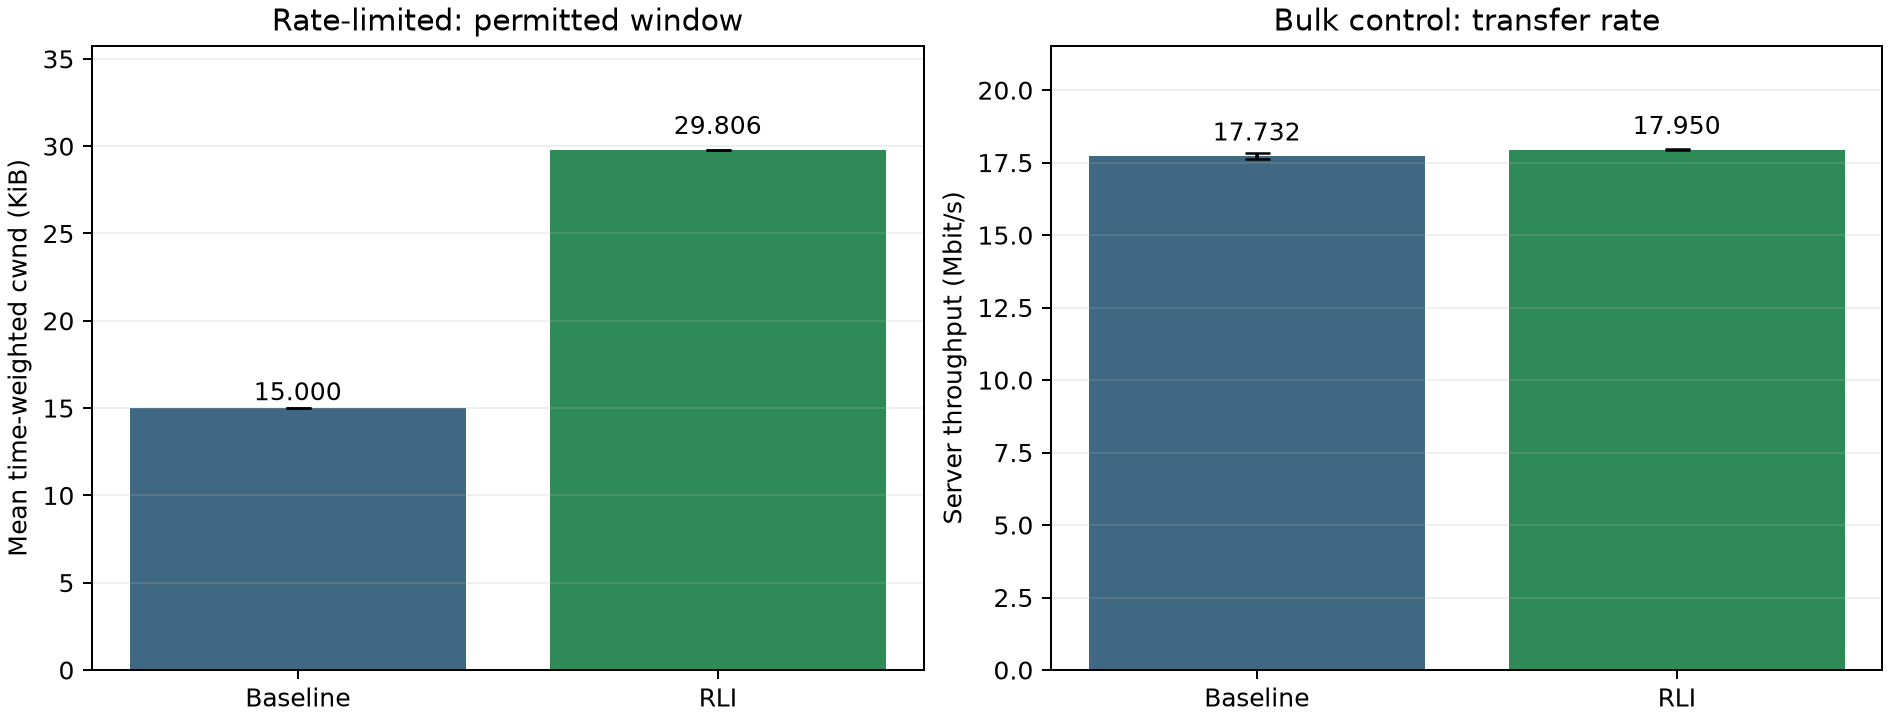
\includegraphics[width=\textwidth]{plots/overview.png}
\caption{Three-run means with sample standard-deviation error bars.
Left: permitted congestion-window behavior under rate limitation.
Right: bulk-control throughput. These axes measure different quantities.}
\end{figure}

\subsection{What improved}
For the rate-limited workload, baseline mean time-weighted cwnd was
\RateBaselineCwnd{} KiB and RLI mean was \RateRliCwnd{} KiB, an increase
of \WindowChange\%. The final RLI window reaches 30 KiB, compared with
15 KiB for baseline, and stays bounded. This demonstrates the intended
change from suppressed growth to controlled growth for the tested case.

The mean throughputs were \RateBaselineThroughput{} and
\RateRliThroughput{} Mbit/s. Application supply is the limiting factor,
so these measurements do not demonstrate increased useful data delivery.
They also do not measure faster restart after a long idle period or a
large subsequent application burst.

\subsection{Bulk-control interpretation}
Mean bulk throughput changed from \BulkBaselineThroughput{} to
\BulkRliThroughput{} Mbit/s, a \BulkChange\% difference. Small changes
between three local runs can arise from scheduling, queueing, ACK timing,
and the original CUBIC dynamics. The per-run table and CSV, including
retransmission counts, provide the basis for the control comparison.
The report does not label a small mean difference as a statistically
proven speed gain.

Connection duration in the tables comes from the server performance CSV.
The qlog metric span is separately retained in \path{measurements.csv}.
Throughput uses the server's sent-byte count divided by its connection
duration, with decimal Mbit/s units. Cwnd statistics use reconstructed
metric snapshots and left-step time weighting. The analysis includes the
logger's initial zero cap-flag interval when computing cap fractions;
the unadjusted generic helper starts that fraction at its first explicit
flag observation. This adjustment affects cap-duration statistics, not
the cwnd or throughput gains. The final cwnd is state
retained at transfer completion, not remaining outstanding data.

\subsection{Two competing flows on the full dumbbell}
% Generated from the six supplementary dumbbell experiments.
\begin{table}[H]\centering\small
\begin{tabular}{llrrrrr}\toprule
Run & Mode & Flow 1 & Flow 2 & Combined & Jain index & Retrans.\\
 & & (Mbit/s) & (Mbit/s) & (Mbit/s) & & \\\midrule
1 & baseline & 8.737 & 8.734 & 18.669 & 1.000 & 615 \\
1 & rli & 8.743 & 8.781 & 18.680 & 1.000 & 445 \\
2 & baseline & 9.430 & 8.776 & 18.662 & 0.999 & 443 \\
2 & rli & 8.045 & 7.707 & 18.574 & 1.000 & 477 \\
3 & baseline & 8.754 & 8.955 & 18.665 & 1.000 & 292 \\
3 & rli & 8.753 & 8.773 & 18.621 & 1.000 & 376 \\
\bottomrule\end{tabular}
\caption{Two-flow dumbbell results. Flow rates use each server's connection CSV. Combined rate uses both byte counts divided by the common client wall time, including connection completion.}\end{table}
The mean combined wall-time rates were 18.665 Mbit/s for baseline and 18.625 Mbit/s for RLI (-0.22\%). The combined wall interval starts at client launch and ends when both clients exit; it excludes the later wait for server shutdown. The per-flow CSV rates use each server's own connection interval, so their sum is not the combined wall-time rate. The Jain index uses the two per-connection rates; values closer to one indicate a more even split. It describes this pair of flows over their connection lifetimes, not instantaneous fairness or fairness against other congestion algorithms.

Both pairs transmit application data through the shared bottleneck. This
tests competition between two connections using the same congestion-control
mode, rather than competition between different algorithms. The transfer
byte counts are checked at both the sender and receiver, and each RLI
connection's qlog passes the observed-invariant validator.

\section{Graph reading guide and validation verdict}
Every detailed graph uses seconds on the x-axis and KiB on the y-axis.
Blue is cwnd; grey is bytes in flight. RLI plots also show the flight
history, the current growth ceiling, and cap-active markers. Overlapping
curves can conceal a limit line when cwnd equals it.

The six rate-limited plots answer whether growth is allowed and bounded
when application supply is low. The six bulk plots answer whether a
fully loaded connection behaves reasonably with the feature enabled.
They should not be compared solely by window height: the workloads
deliberately provide very different amounts and timing of data. When a
transfer ends, bytes in flight can fall to zero while cwnd remains at its
last value.

All six main RLI qlogs pass the observed-invariant validator. The six
RLI connections in the supplementary dumbbell runs also pass. For the three
rate-limited runs, an active cap is explicitly required; for the bulk
runs, the extra check requires a visible cwnd reduction with a flight-history
reset. The analysis also checks complete JSON, one sender path, expected
transfer byte counts, CSV throughput arithmetic, and baseline traces
without RLI metrics.

\textbf{Verdict: the output is correct for the checked conditions and the
implemented limits.} Both builds and registered test suites pass, the
focused test passes, the rate-limited growth is bounded as intended,
and the new experiments support the reported measurements. This is a
scoped verification verdict, not a proof of complete IETF conformance or
all-network performance improvement.

\subsection{Limitations and further work}
The experiments use one bottleneck capacity, one base delay, two workloads,
and three repetitions per configuration. Additional tests should cover
application bursts after idle, receiver flow-control limitation, longer
idle periods, competition with different congestion algorithms, multiple paths, variable delay,
and deliberately injected loss/ECN. Unit assertions exercise congestion
notifications but are not equivalent to all those end-to-end conditions.

The qlog records metric snapshots and can miss intermediate flight peaks;
the validator checks what is observable rather than inventing hidden
events. The report does not claim that per-path storage itself proves
multipath correctness, that overflow boundary cases were independently
tested, or that the fixed additive CA ceiling fully resolves the draft's
general time-based CUBIC interpretation. Long-term cwnd decay and RFC 7661
window validation remain separate topics. More repetitions and a wider
test matrix are needed to quantify performance benefits reliably.

\section{Conclusion}
The project adds an opt-in RLI mode to picoquic CUBIC and exposes enough
state to inspect its operation. The implementation passes the registered
regression suites and its focused behavior checks. In the low-rate workload,
it permits ACK-driven growth from 15 KiB to a bounded 30 KiB window;
the application rate remains essentially unchanged. Bulk and competing-flow
experiments provide control measurements under greater offered load.
The supported result is controlled window growth with measured behavior
under the stated conditions. Further test configurations and independent
review are needed before broader conformance or performance claims.

\section{Reproduction and evidence layout}
Run commands from the repository root. The helper scripts save complete
logs and generate tables from raw data instead of manually typed values:
\begin{lstlisting}[language=bash]
cd /home/aryy_02/Desktop/OSNT_Project
python3 "results 1/run_tests.py"
unshare --user --map-root-user --net --mount \
  bash "results 1/run_experiments.sh"
.venv/bin/python "results 1/analyze_results.py"
.venv/bin/python "results 1/analyze_dumbbell.py"
cd "results 1"
../.local-deps/report-tools/tectonic --keep-logs report.tex
pdfinfo report.pdf
pdftotext report.pdf report-extracted.txt
\end{lstlisting}
The helper assumes the local dependencies documented in the README; a
fresh computer should first build picoquic and install the Python plot
requirements. Tectonic downloads standard TeX resources on first use.
An installed TeX Live distribution can alternatively run
\code{pdflatex report.tex} twice from this folder.

\begin{tabularx}{\textwidth}{lX}\toprule
Artifact & Purpose\\\midrule
\path{report.tex}, \path{report.pdf} & Editable LaTeX report and compiled output.\\
\path{generated-*.tex} & Automatically derived numbers, tables, and graph pages.\\
\path{tests/} & Build, CTest, focused-test logs, and detailed CTest records.\\
\path{runs/} & All twelve fresh experiment records, qlogs, CSVs, and plots.\\
\path{dumbbell/} & Six two-flow experiments, twelve transfers, and supplementary metrics.\\
\path{plots/} & Twelve main graphs, one overview, and six competing-flow graphs.\\
\path{raw-evidence.tar.gz} & Lossless archive of all raw experiment records.\\
\path{comparisons/}, \path{validation/} & Pairwise CSVs and trace checks.\\
\path{environment.json} & Linux/compiler details, commits, and binary hashes.\\
\path{measurements.csv}, \path{summary.json} & Machine-readable measurements and aggregates.\\
\path{README.md} & Output correctness assessment and reproduction instructions.\\
\path{SHA256SUMS} & Portable file-integrity manifest for the evidence bundle.\\
\bottomrule\end{tabularx}

\section*{Acknowledgements and tools}
\addcontentsline{toc}{section}{Acknowledgements and tools}
This work builds on the picoquic library and the referenced IETF
specifications. Existing library functionality remains attributable to
its contributors. CMake, CTest, Linux network namespaces, Python,
matplotlib, and LaTeX were used for building, measurement, and reporting.
The conclusions are supported by the archived source revisions and measured
outputs described in this report.

\clearpage
\begin{thebibliography}{9}
\bibitem{rli} M. Welzl, T. Henderson, G. Fairhurst, and M. P. Tahiliani.
\emph{Increase of the Congestion Window when the Sender Is Rate-Limited}.
IETF CCWG, draft-ietf-ccwg-ratelimited-increase-11, September 2026.
Work in progress. \url{https://datatracker.ietf.org/doc/html/draft-ietf-ccwg-ratelimited-increase-11}
\bibitem{quic} J. Iyengar and M. Thomson. \emph{QUIC: A UDP-Based Multiplexed
and Secure Transport}. RFC 9000, May 2021.
\url{https://www.rfc-editor.org/rfc/rfc9000.html}
\bibitem{quiccc} J. Iyengar and I. Swett. \emph{QUIC Loss Detection and
Congestion Control}. RFC 9002, May 2021.
\url{https://www.rfc-editor.org/rfc/rfc9002.html}
\bibitem{cubic} L. Xu et al. \emph{CUBIC for Fast and Long-Distance Networks}.
RFC 9438, August 2023. \url{https://www.rfc-editor.org/rfc/rfc9438.html}
\bibitem{picoquic} Private Octopus contributors. \emph{picoquic source repository}.
\url{https://github.com/private-octopus/picoquic}
Project fork: \url{https://github.com/yoman12357/OSNT_Project}
\end{thebibliography}

\appendix
\clearpage
\section{All twelve fresh congestion-window graphs}
Each page below contains a matched baseline/RLI pair from one repetition.
The captions give measurements from that exact run. Repetition is used
to check consistency, not to imply a different algorithm or test class.
\subsection{Rate-limited, repetition 1}
\begin{figure}[H]\centering
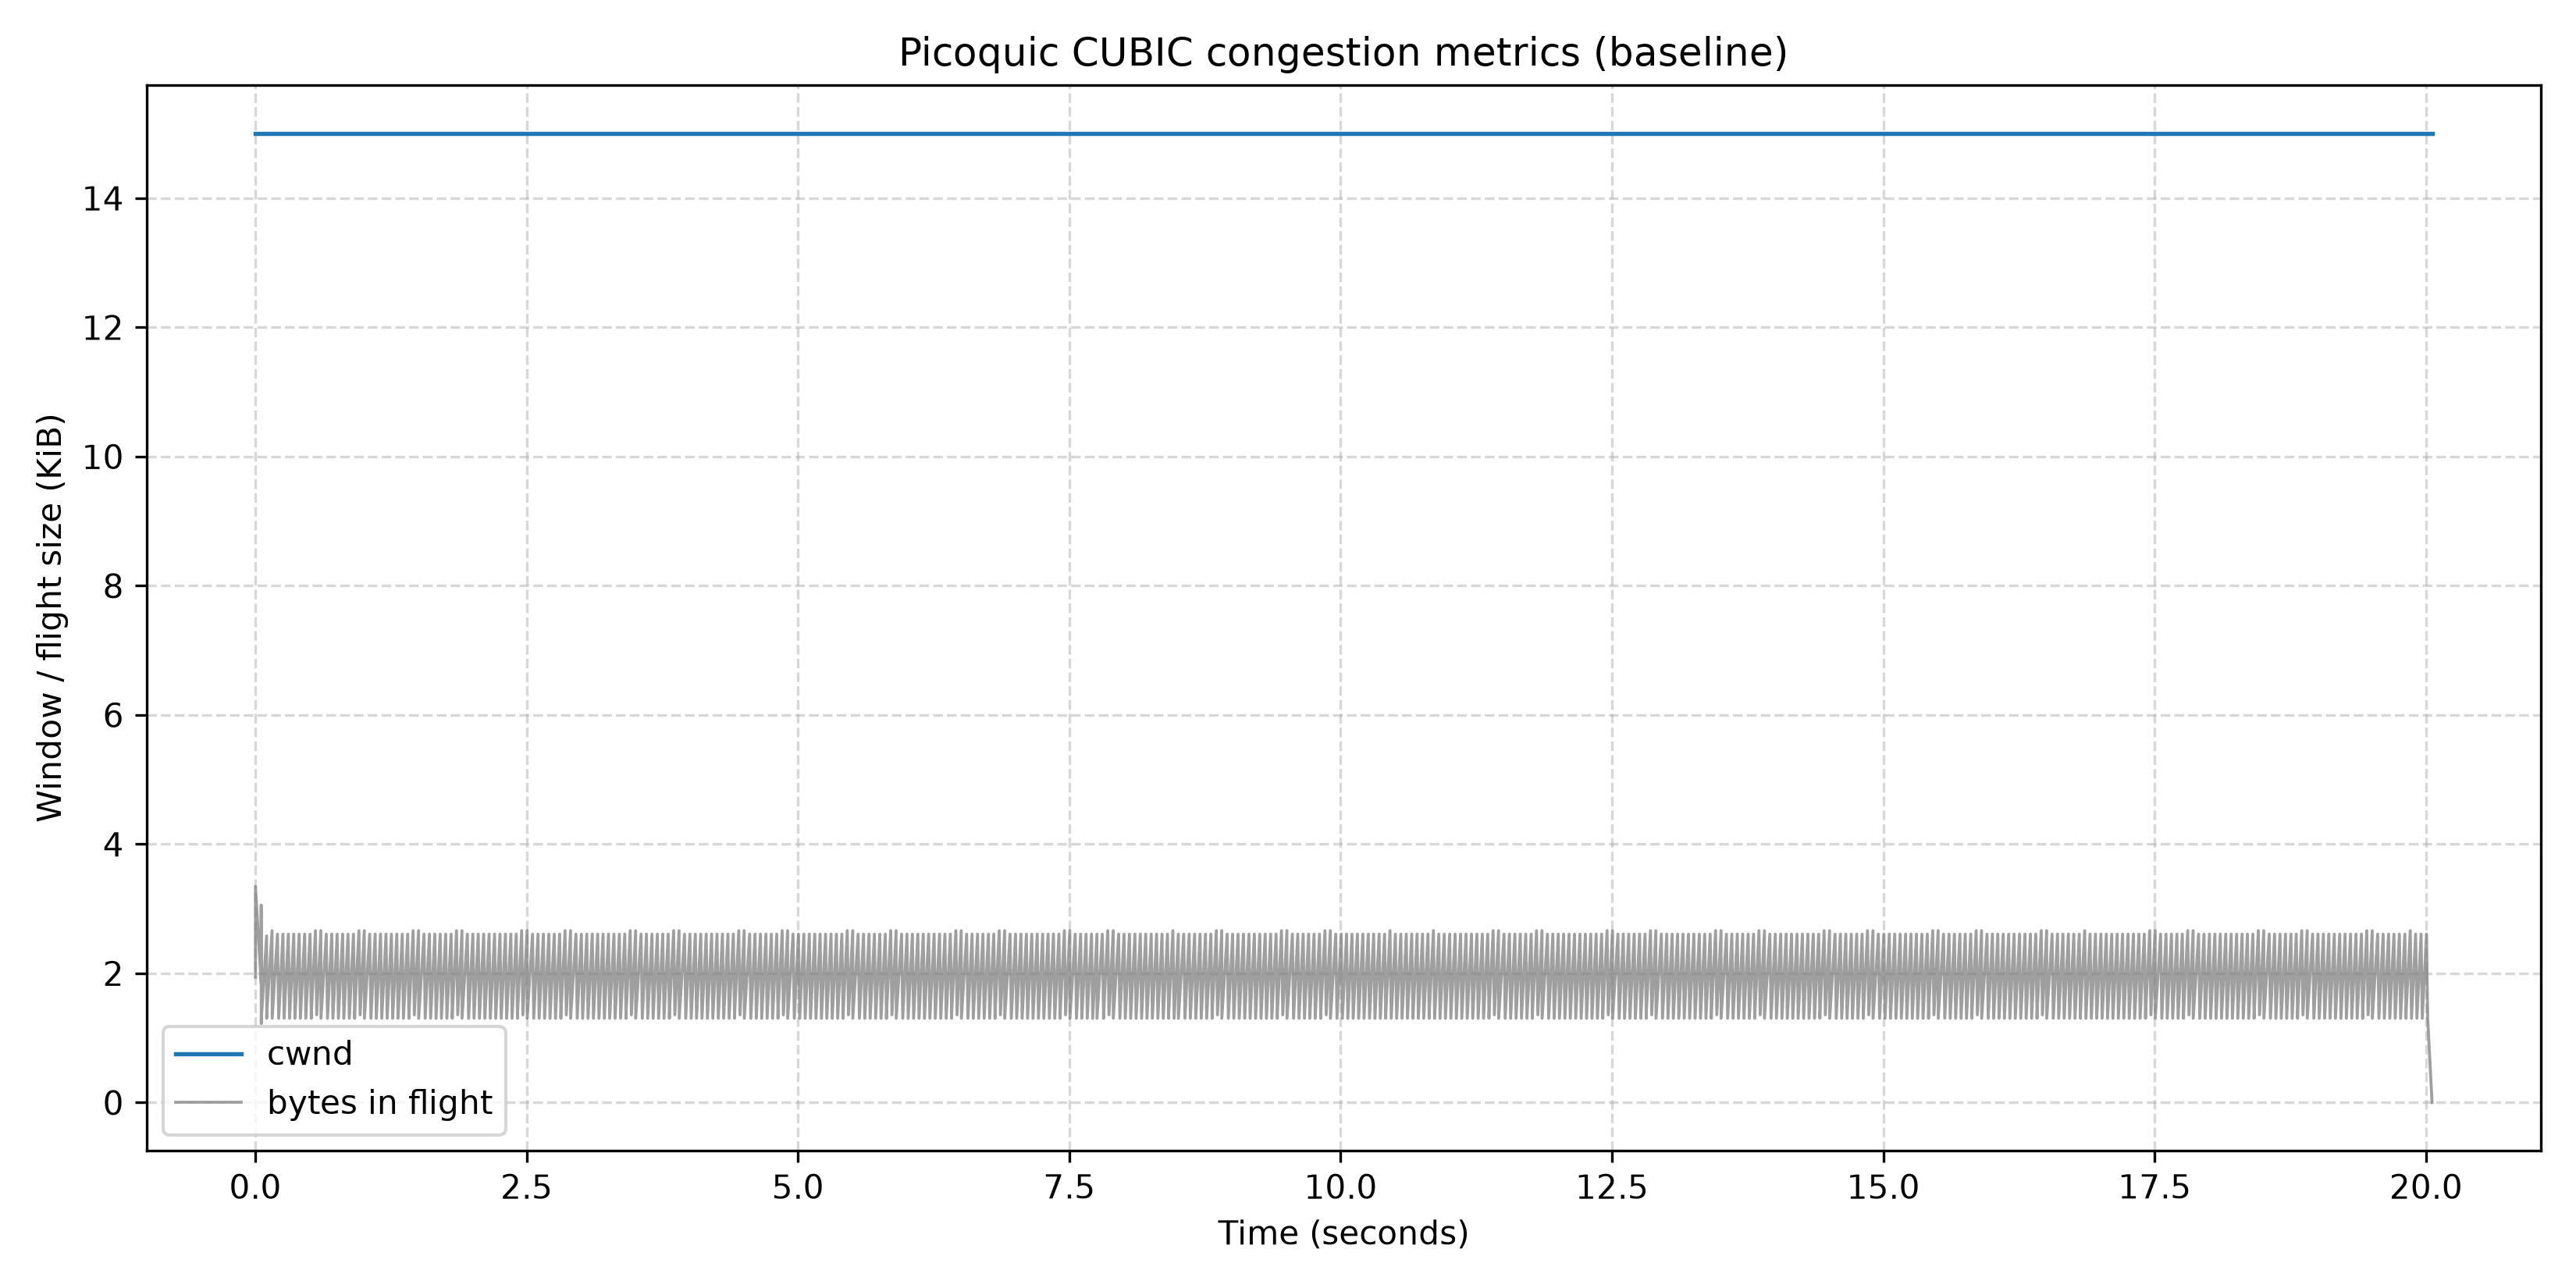
\includegraphics[width=0.92\textwidth]{plots/rate-limited-baseline-1.png}
\caption{Baseline: final cwnd 15.00 KiB; time-weighted mean 15.00 KiB; throughput 0.190 Mbit/s.}\end{figure}
\begin{figure}[H]\centering
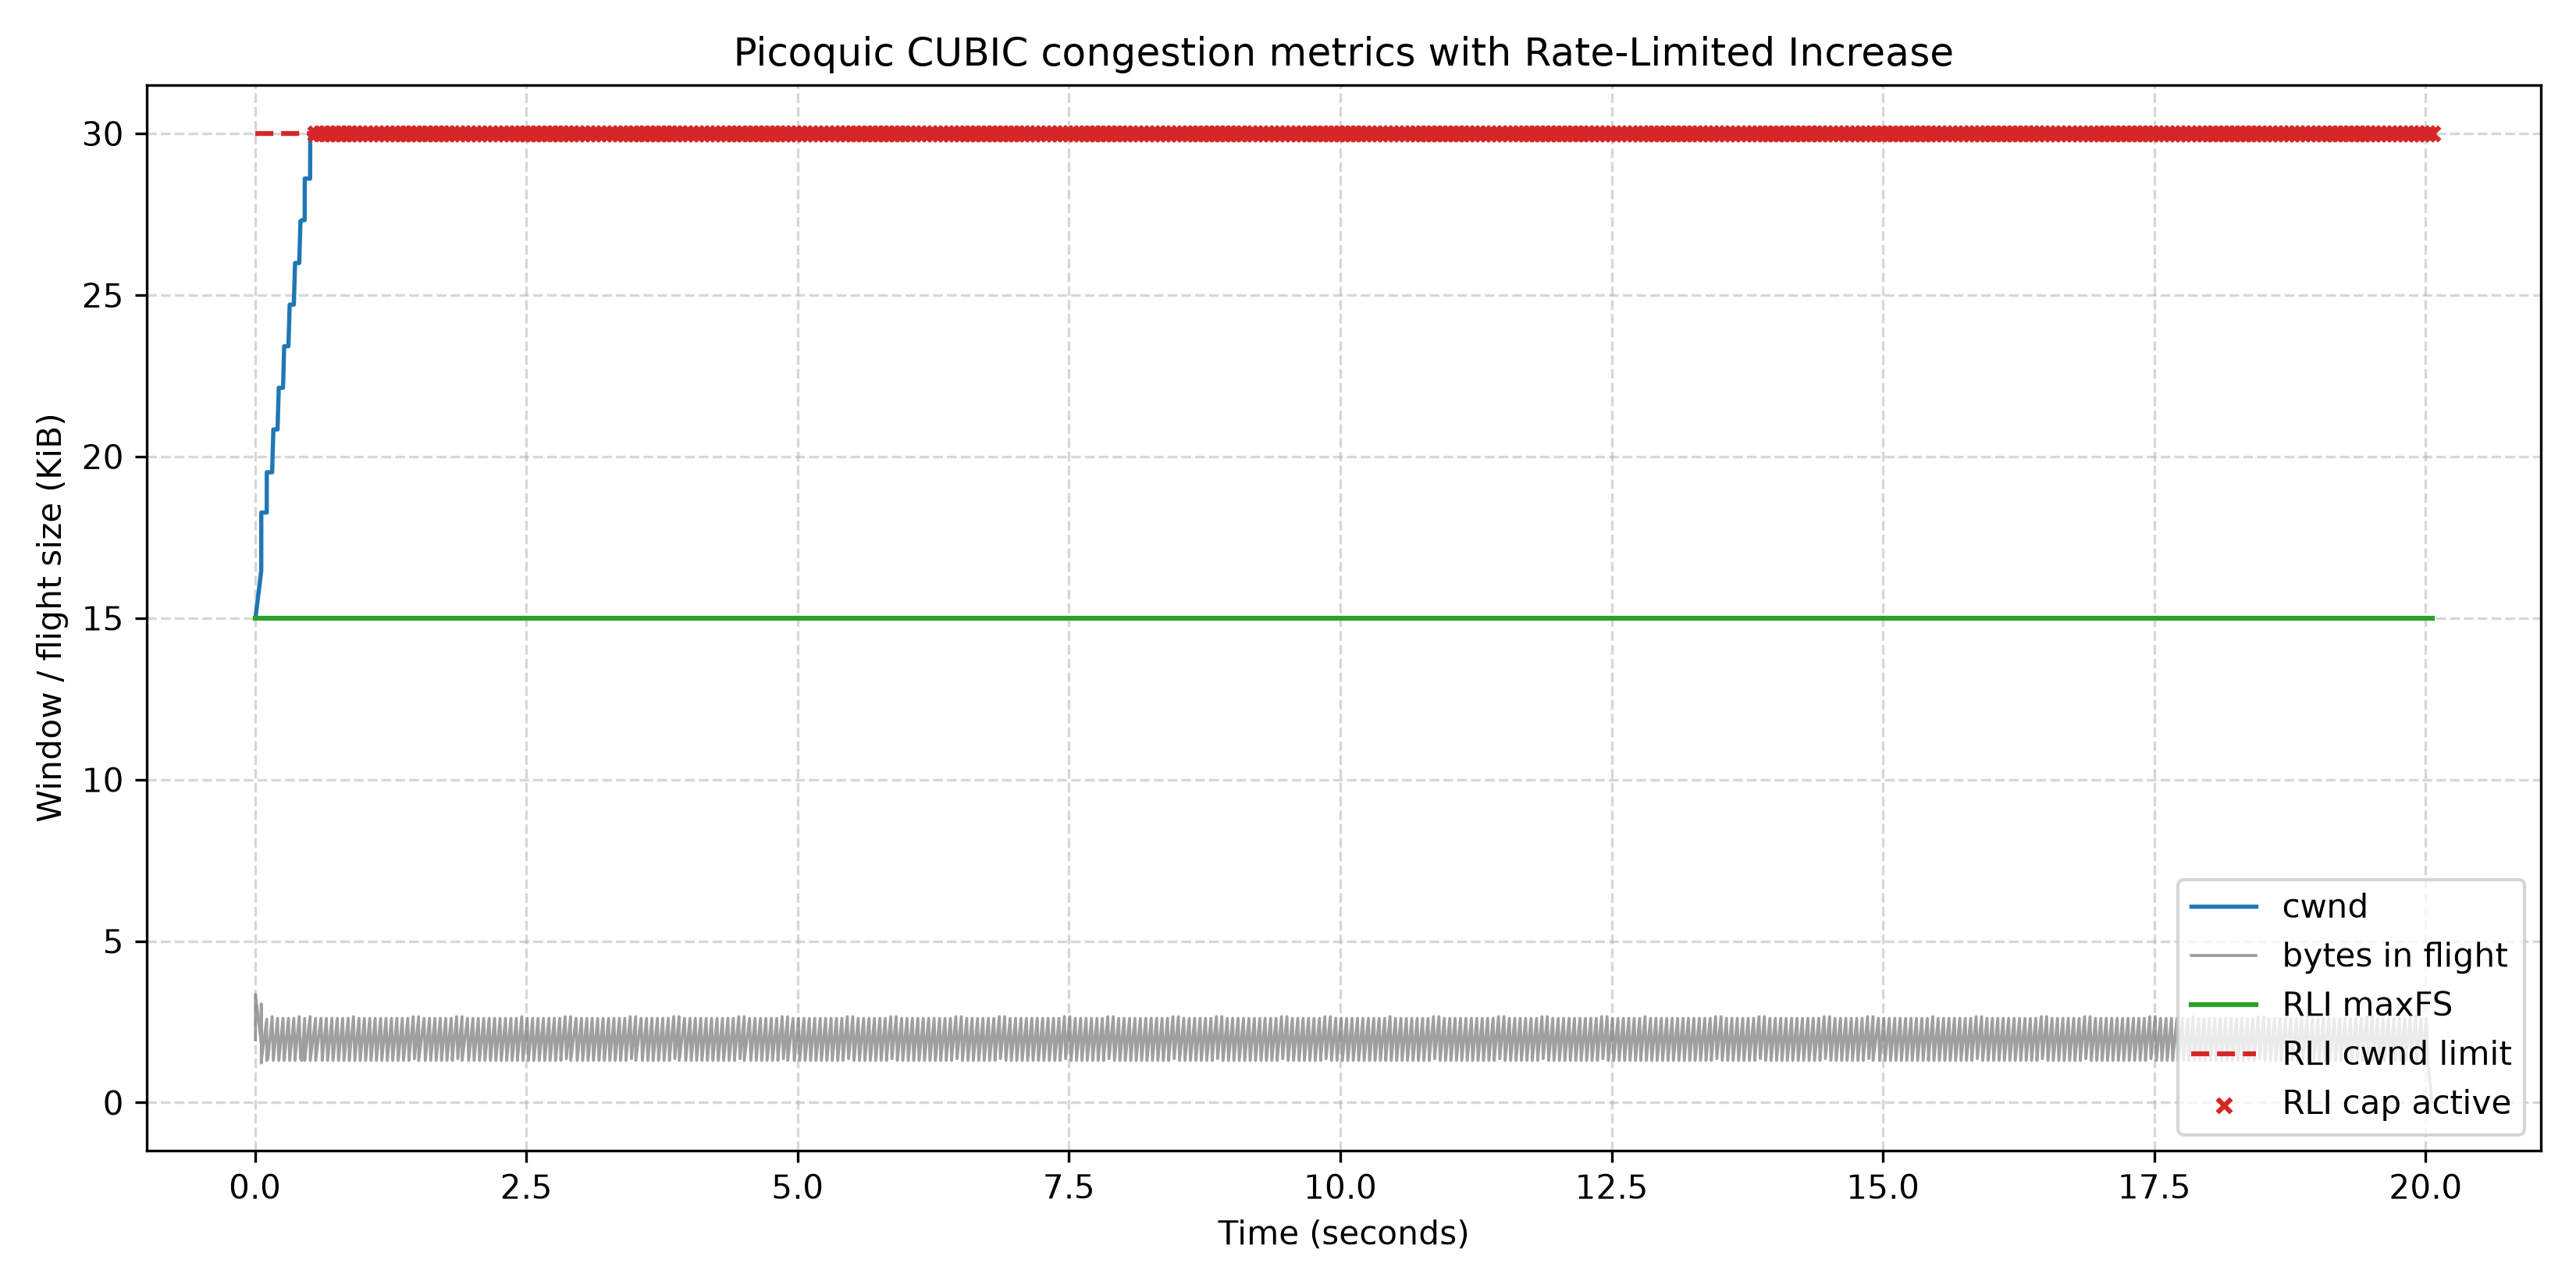
\includegraphics[width=0.92\textwidth]{plots/rate-limited-rli-1.png}
\caption{Rli: final cwnd 30.00 KiB; time-weighted mean 29.81 KiB; throughput 0.190 Mbit/s.}\end{figure}
These matched traces isolate rate-limited window growth. RLI permits bounded ACK-driven growth; application supply still controls throughput.
\clearpage\subsection{Rate-limited, repetition 2}
\begin{figure}[H]\centering
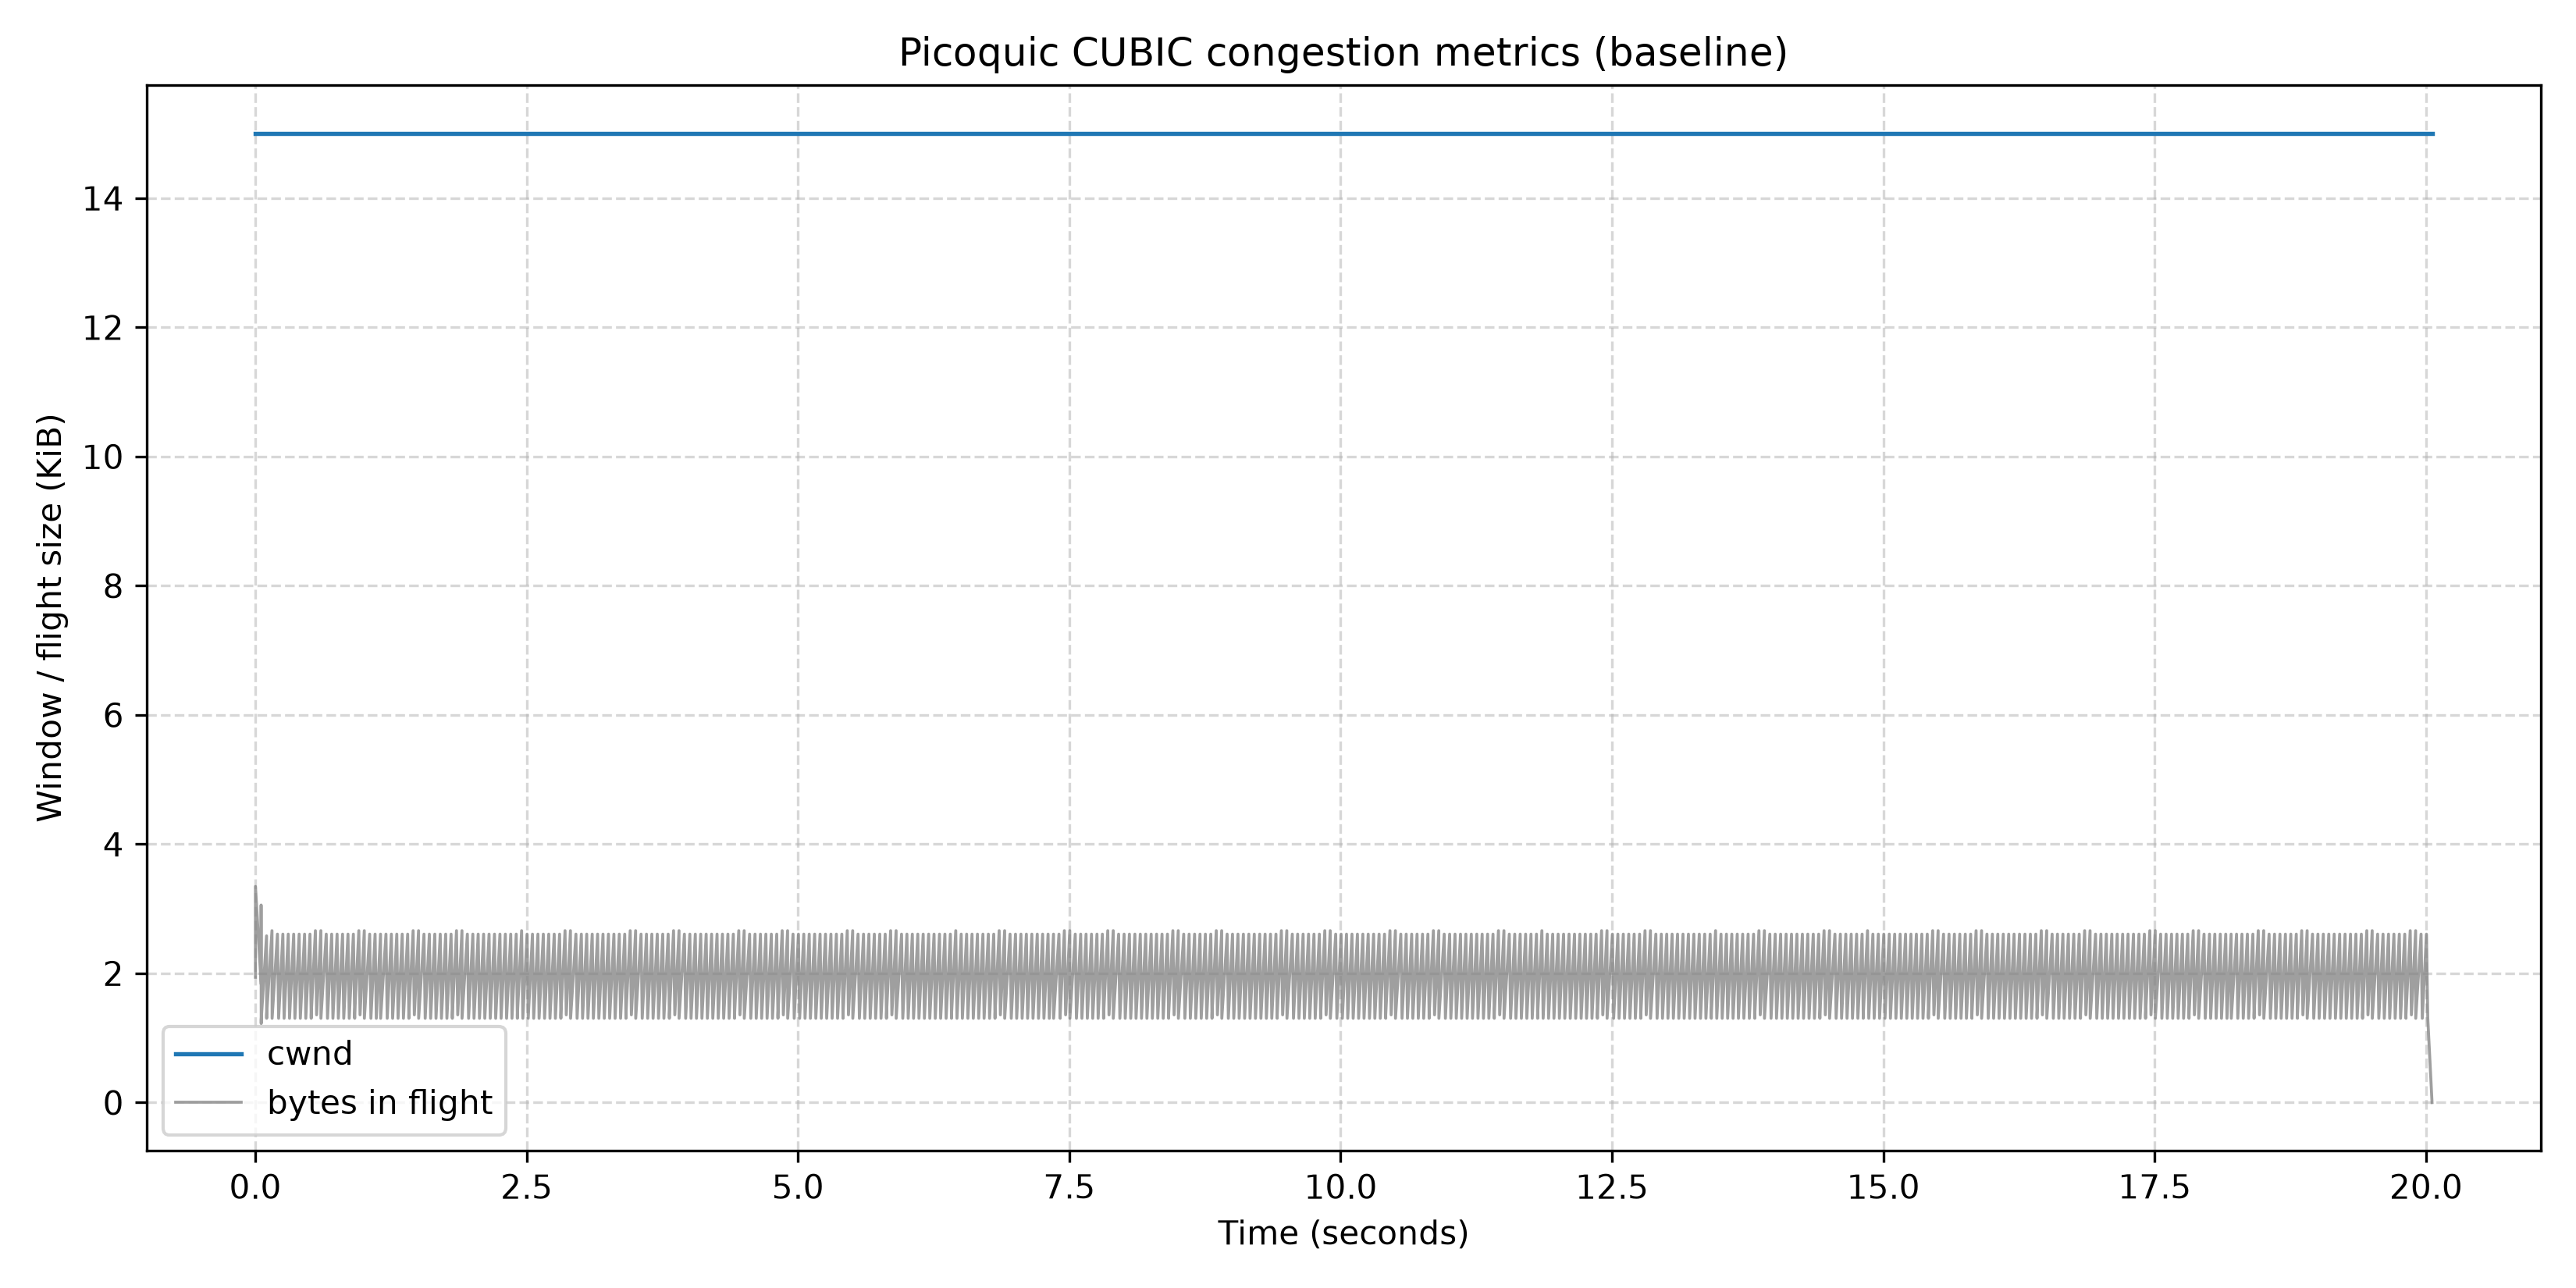
\includegraphics[width=0.92\textwidth]{plots/rate-limited-baseline-2.png}
\caption{Baseline: final cwnd 15.00 KiB; time-weighted mean 15.00 KiB; throughput 0.190 Mbit/s.}\end{figure}
\begin{figure}[H]\centering
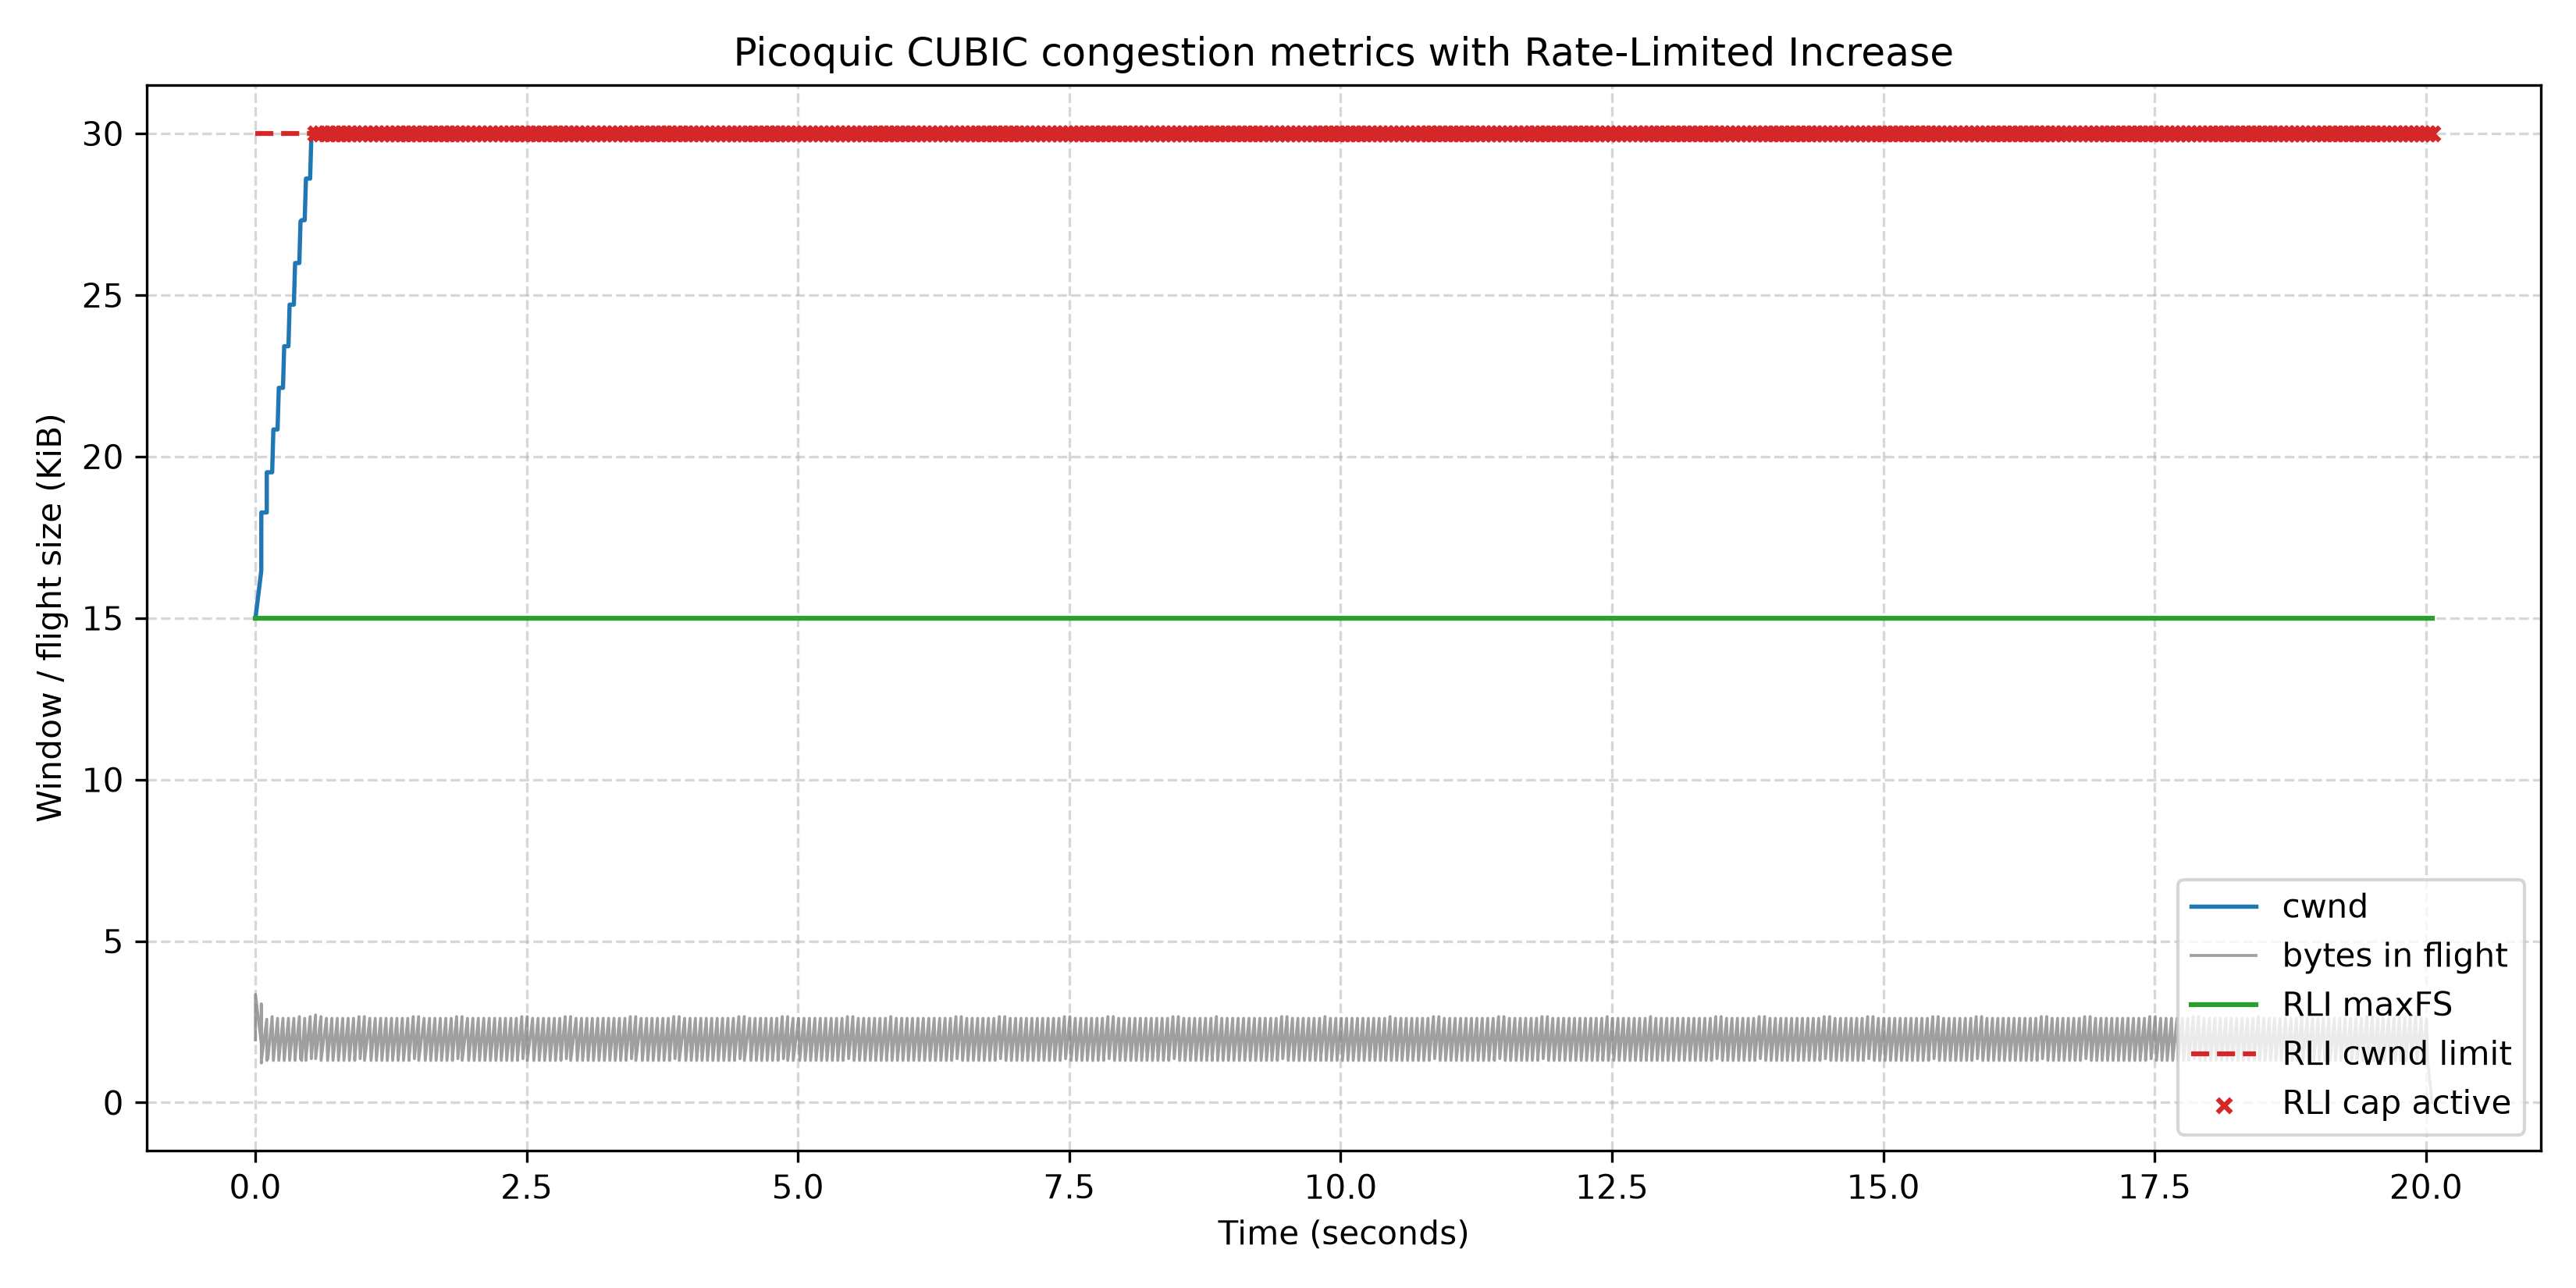
\includegraphics[width=0.92\textwidth]{plots/rate-limited-rli-2.png}
\caption{Rli: final cwnd 30.00 KiB; time-weighted mean 29.81 KiB; throughput 0.190 Mbit/s.}\end{figure}
These matched traces isolate rate-limited window growth. RLI permits bounded ACK-driven growth; application supply still controls throughput.
\clearpage\subsection{Rate-limited, repetition 3}
\begin{figure}[H]\centering
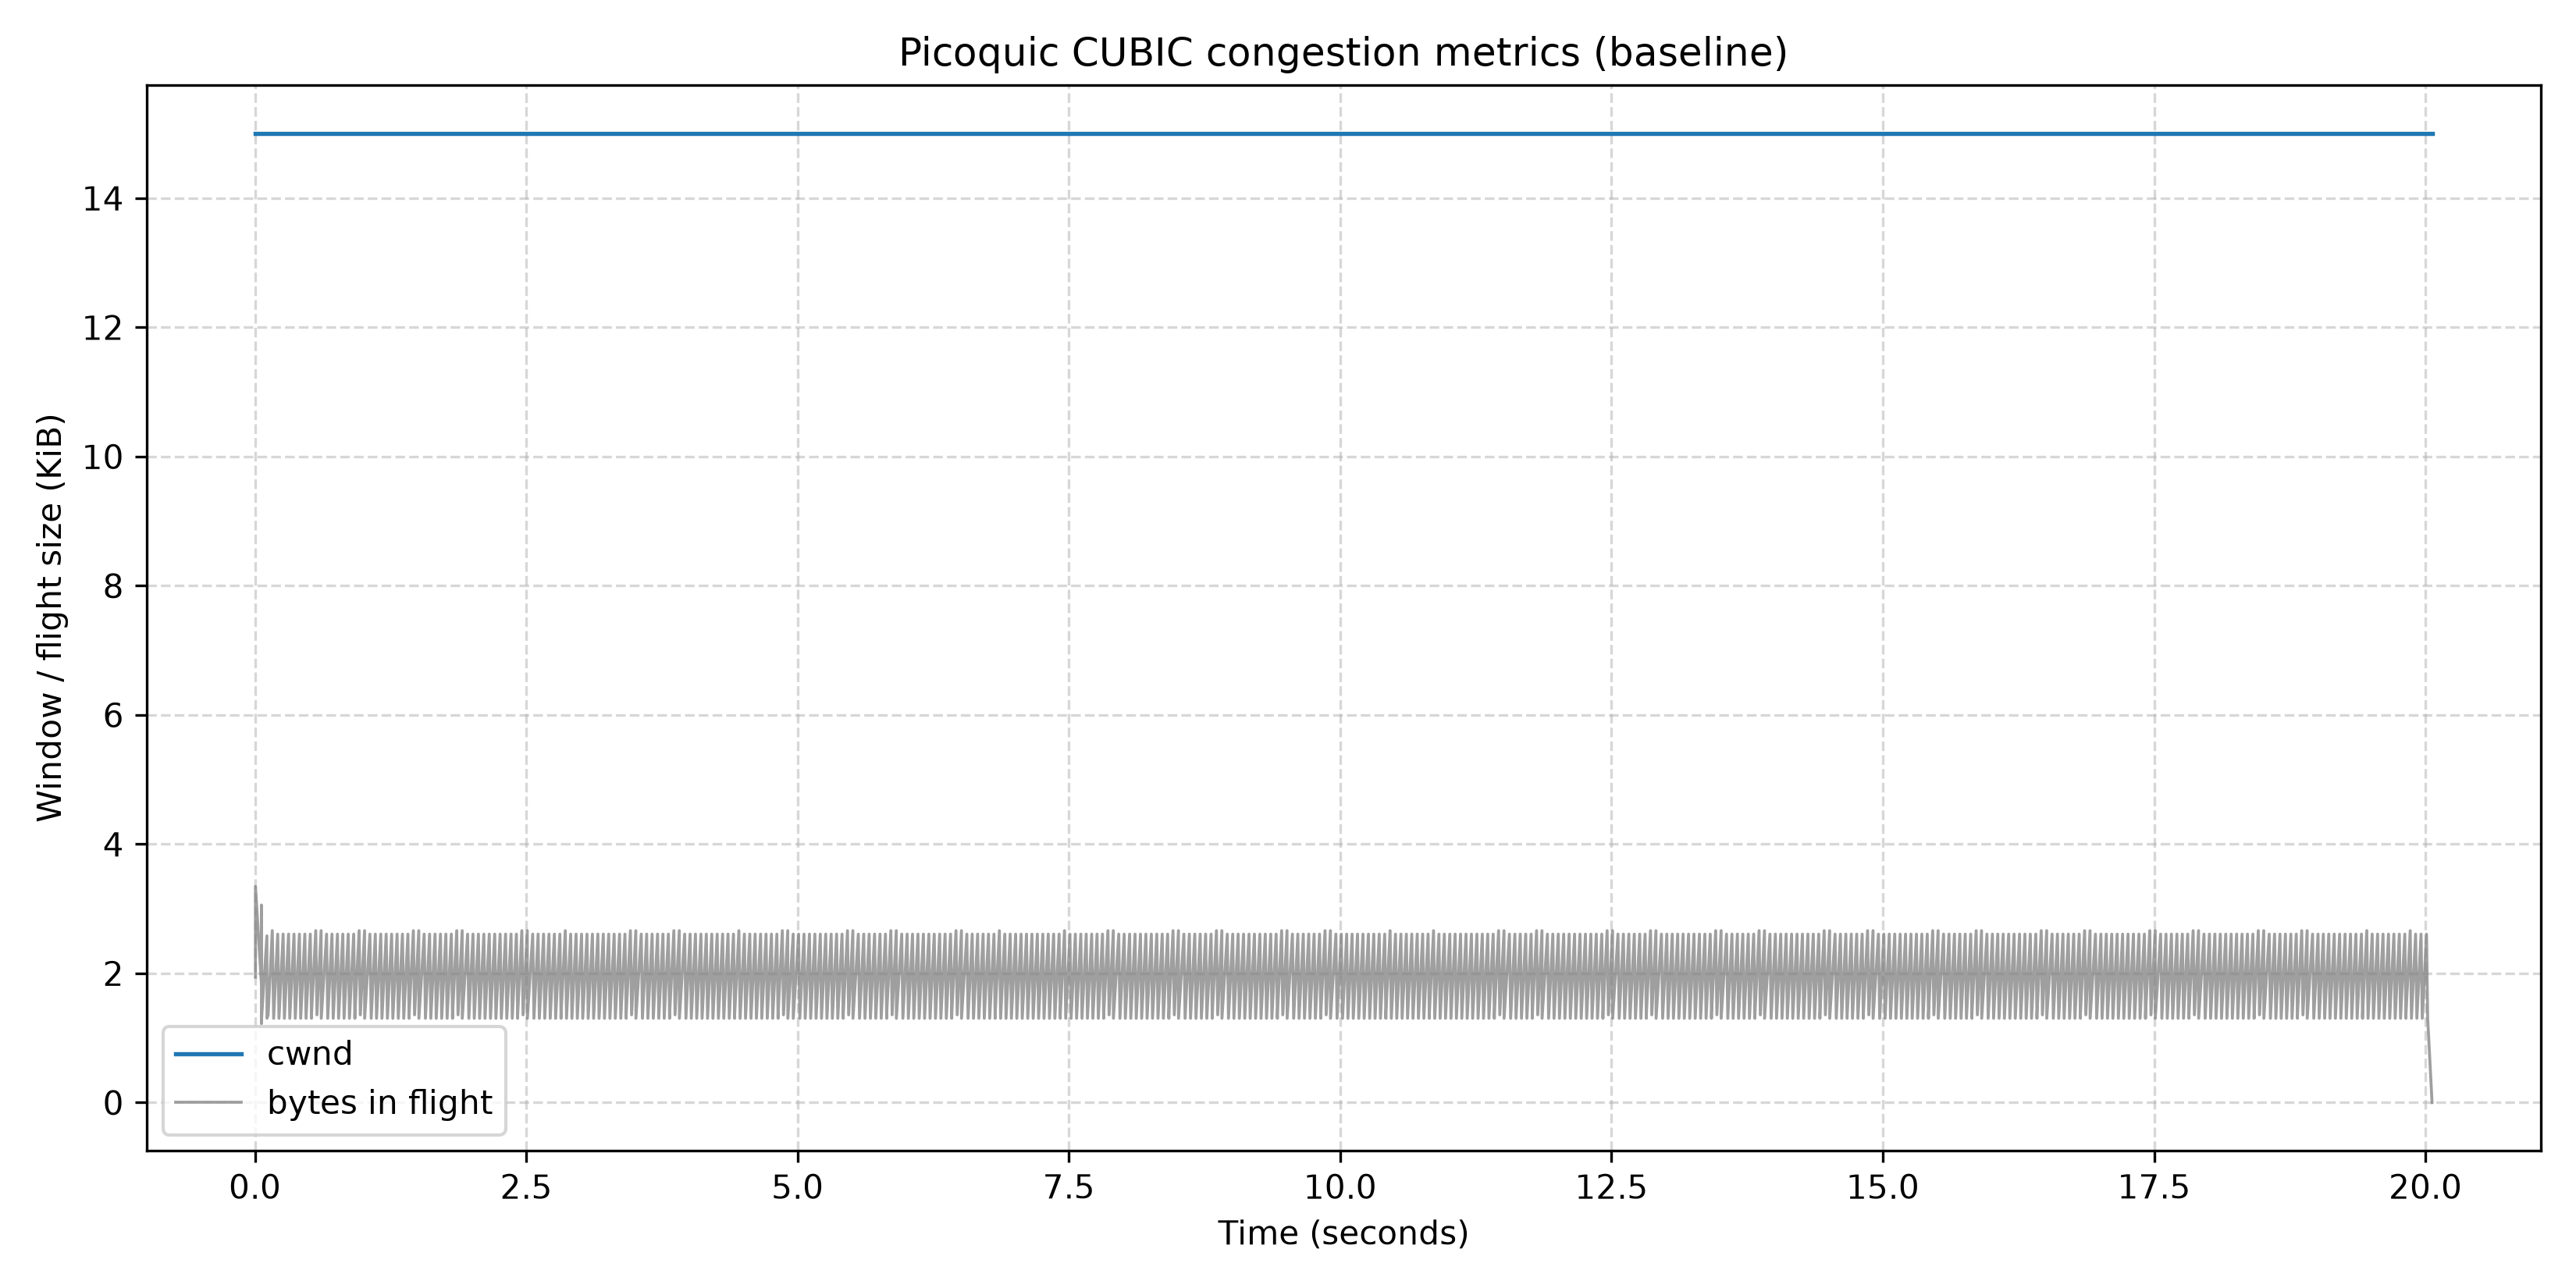
\includegraphics[width=0.92\textwidth]{plots/rate-limited-baseline-3.png}
\caption{Baseline: final cwnd 15.00 KiB; time-weighted mean 15.00 KiB; throughput 0.190 Mbit/s.}\end{figure}
\begin{figure}[H]\centering
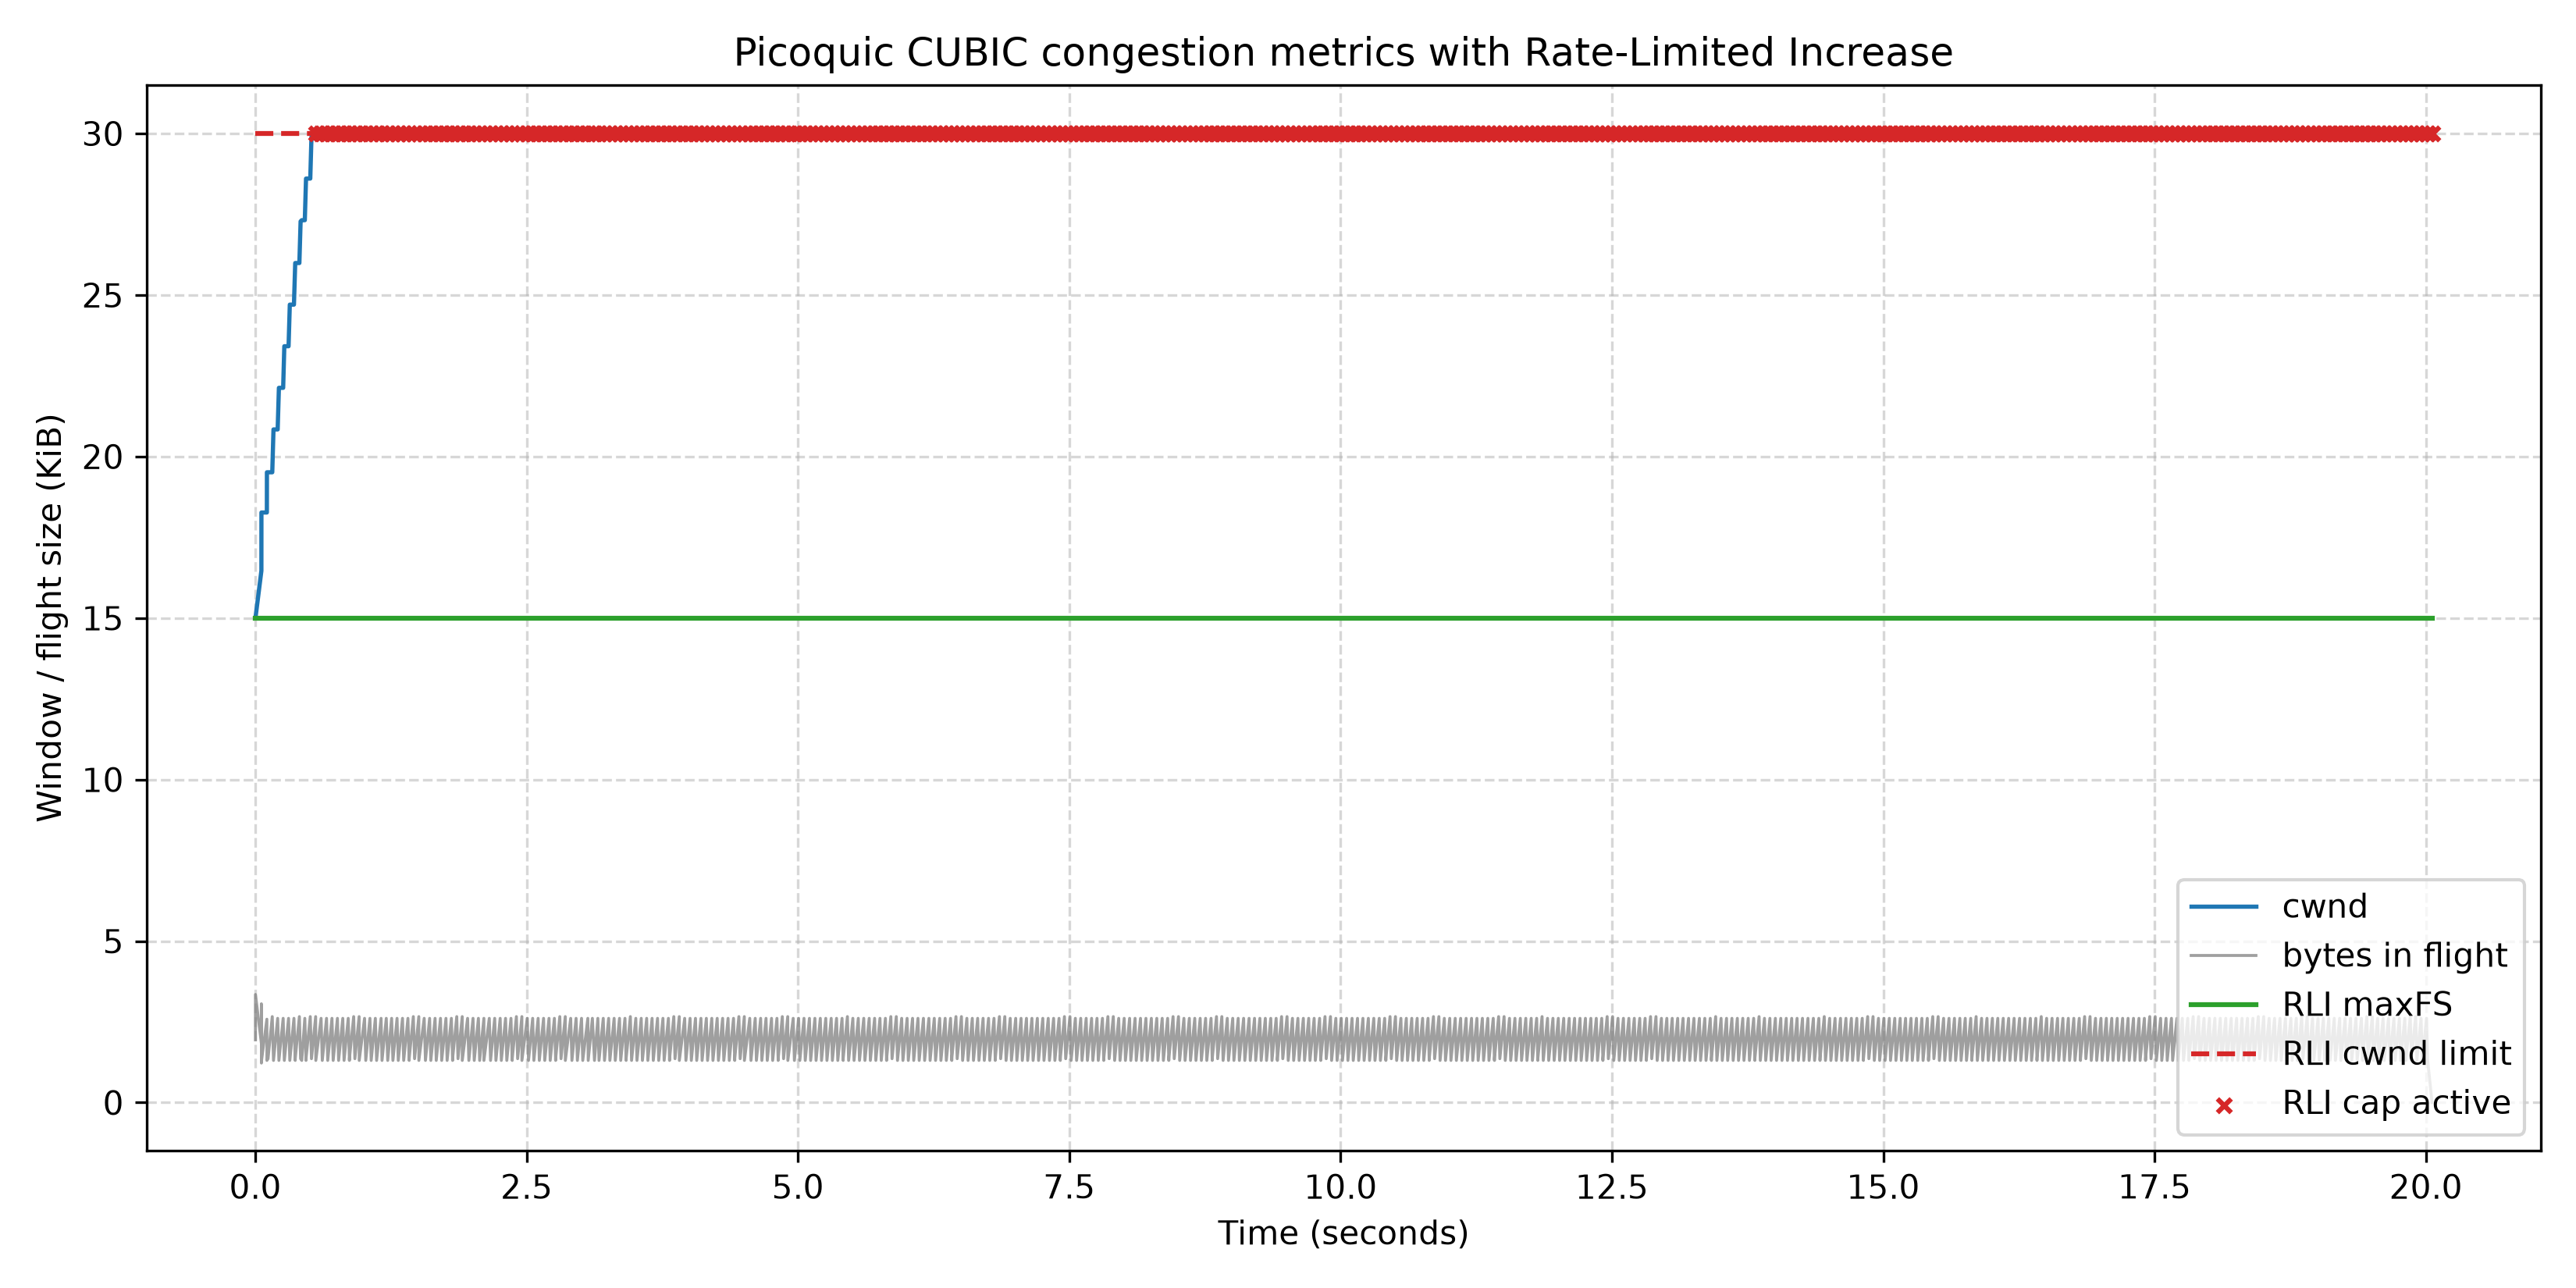
\includegraphics[width=0.92\textwidth]{plots/rate-limited-rli-3.png}
\caption{Rli: final cwnd 30.00 KiB; time-weighted mean 29.81 KiB; throughput 0.190 Mbit/s.}\end{figure}
These matched traces isolate rate-limited window growth. RLI permits bounded ACK-driven growth; application supply still controls throughput.
\clearpage\subsection{Bulk control, repetition 1}
\begin{figure}[H]\centering
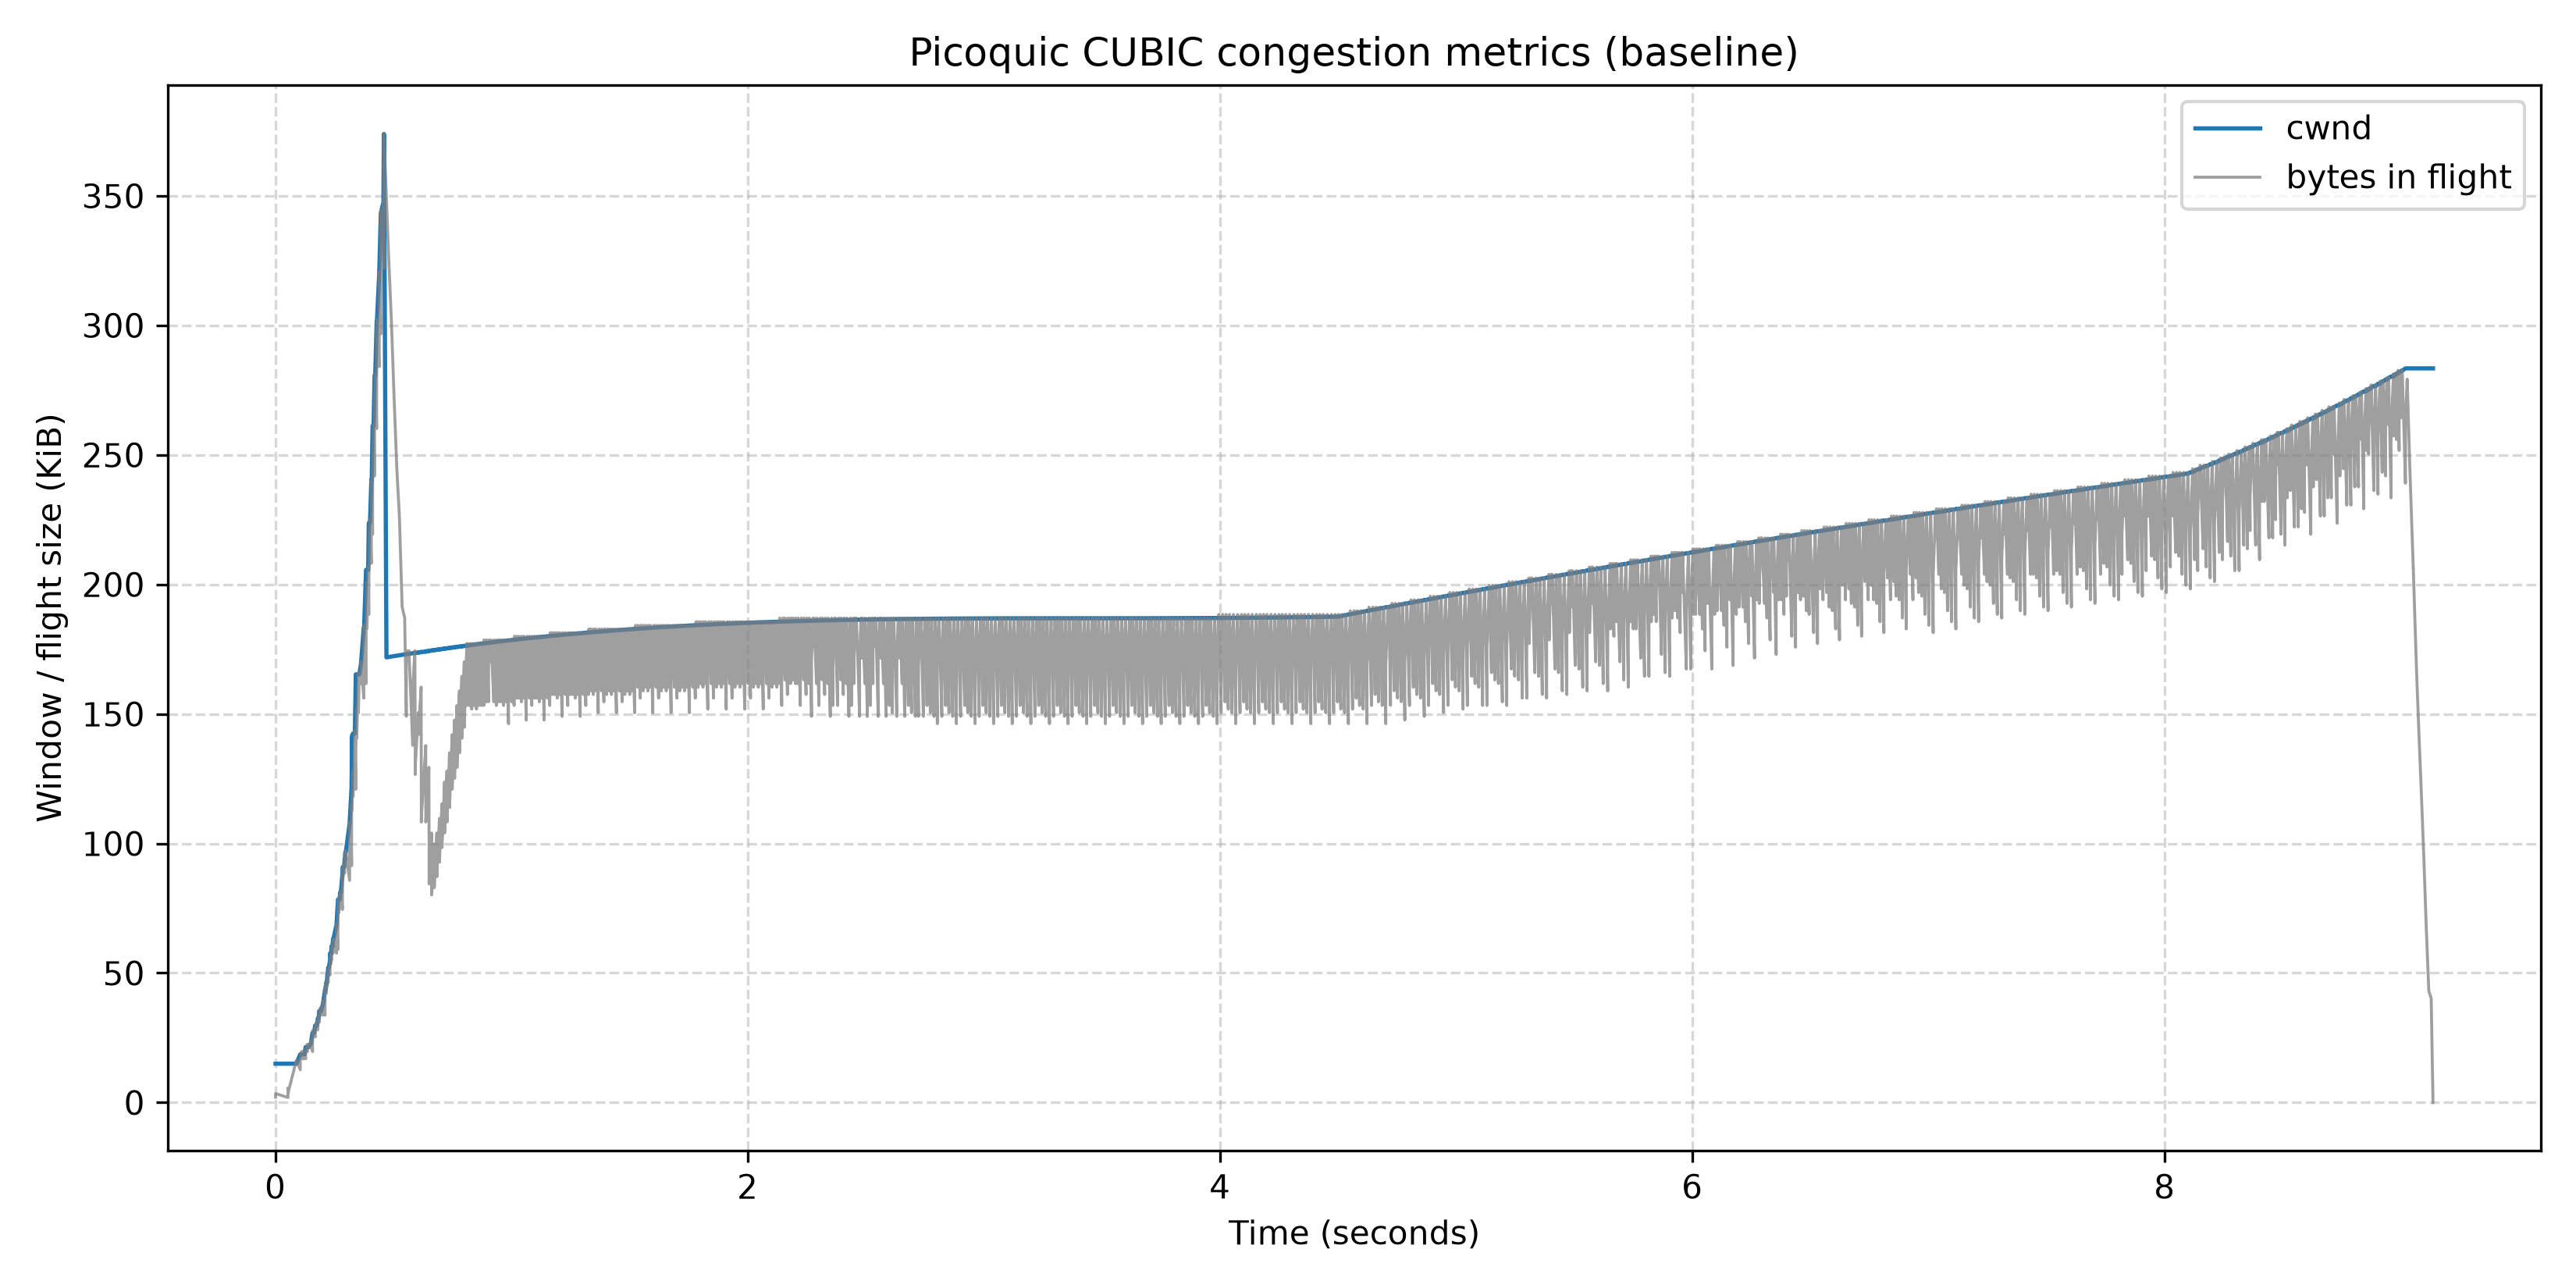
\includegraphics[width=0.92\textwidth]{plots/bulk-baseline-1.png}
\caption{Baseline: final cwnd 283.41 KiB; time-weighted mean 201.63 KiB; throughput 17.731 Mbit/s.}\end{figure}
\begin{figure}[H]\centering
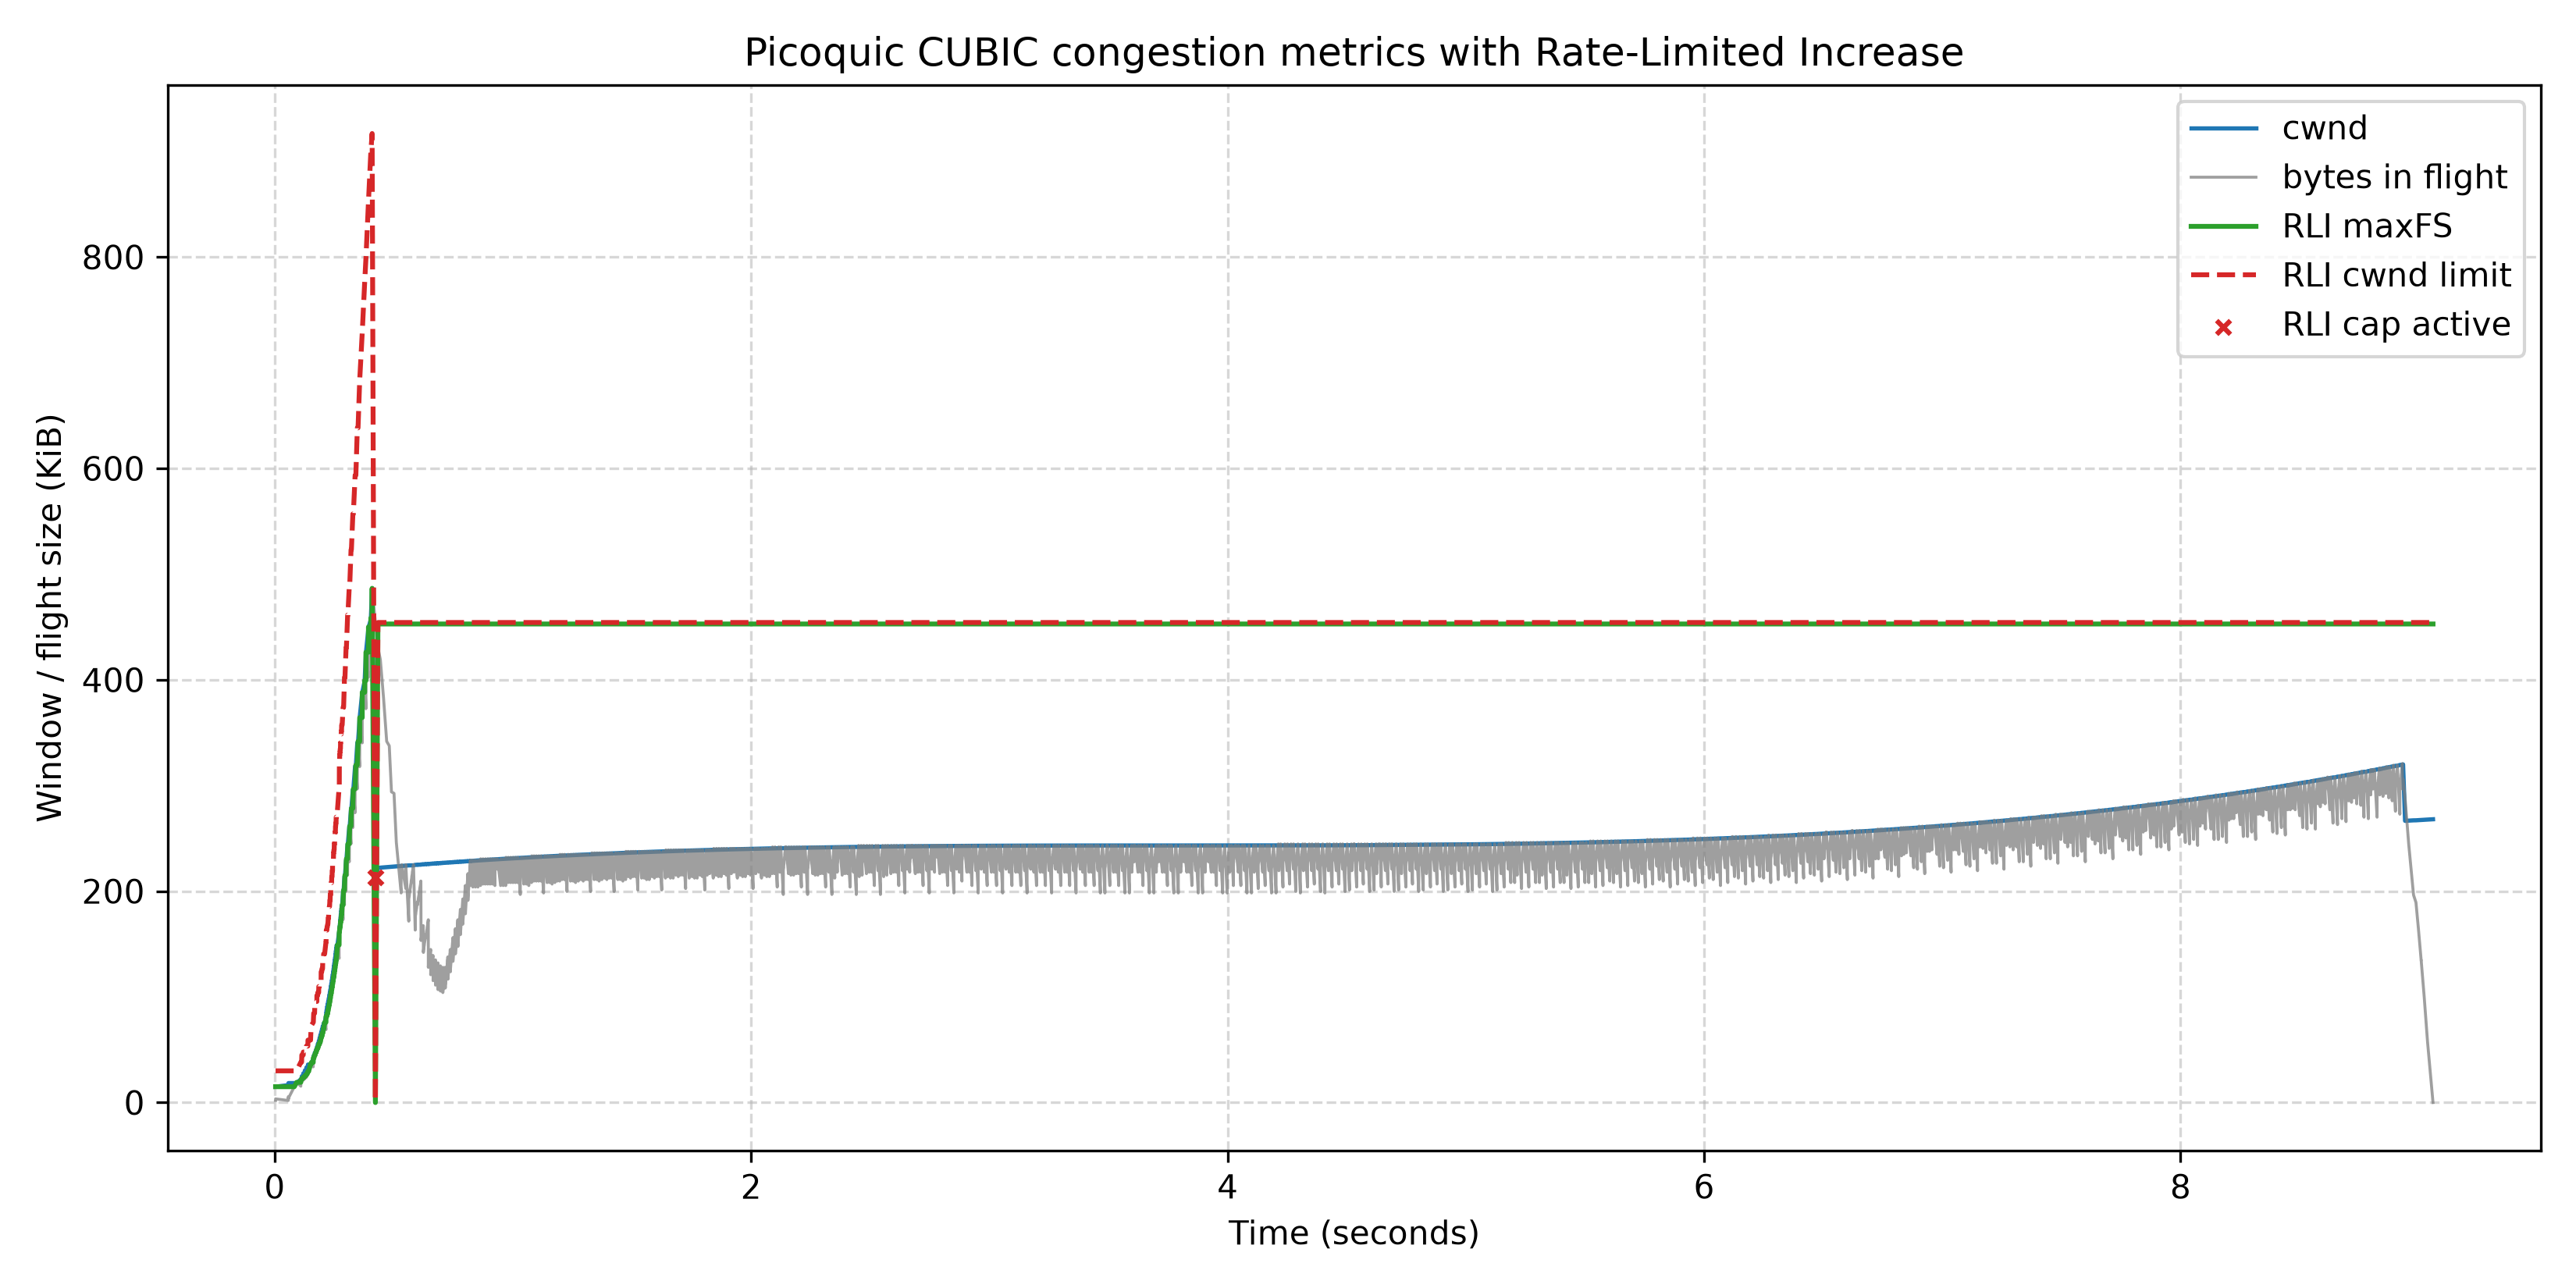
\includegraphics[width=0.92\textwidth]{plots/bulk-rli-1.png}
\caption{Rli: final cwnd 268.04 KiB; time-weighted mean 248.21 KiB; throughput 17.940 Mbit/s.}\end{figure}
These matched traces test a continuously backlogged sender. Normal CUBIC growth and congestion responses dominate; compare measured throughput rather than window height alone.
\clearpage\subsection{Bulk control, repetition 2}
\begin{figure}[H]\centering
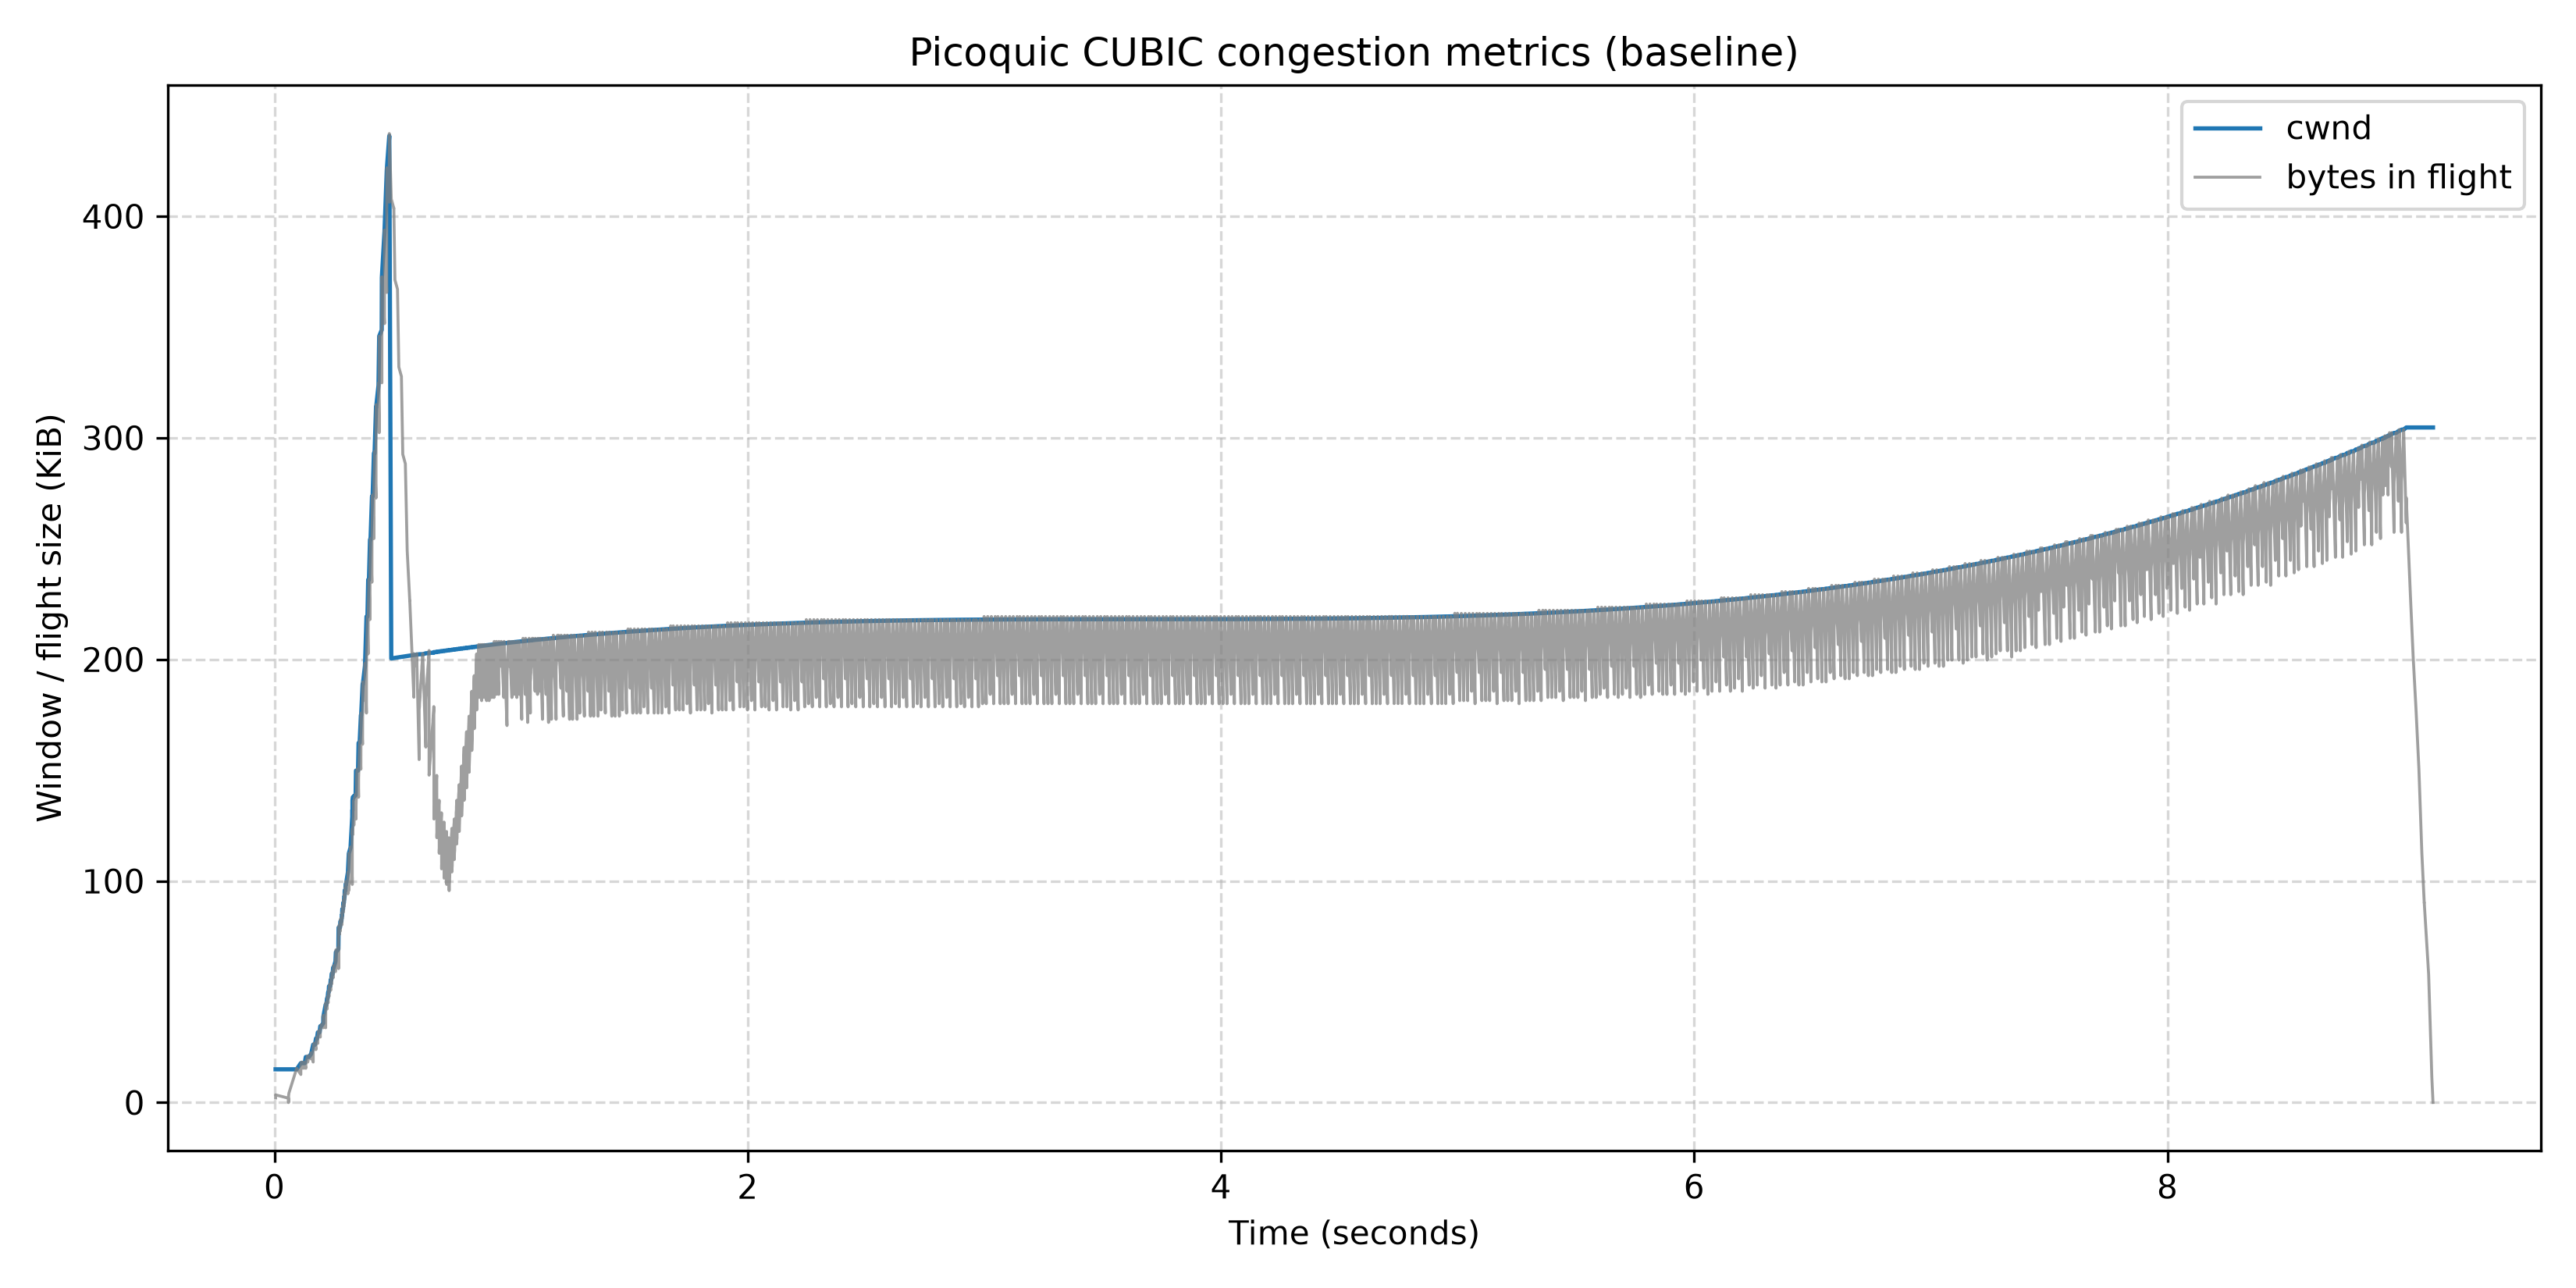
\includegraphics[width=0.92\textwidth]{plots/bulk-baseline-2.png}
\caption{Baseline: final cwnd 304.68 KiB; time-weighted mean 224.90 KiB; throughput 17.823 Mbit/s.}\end{figure}
\begin{figure}[H]\centering
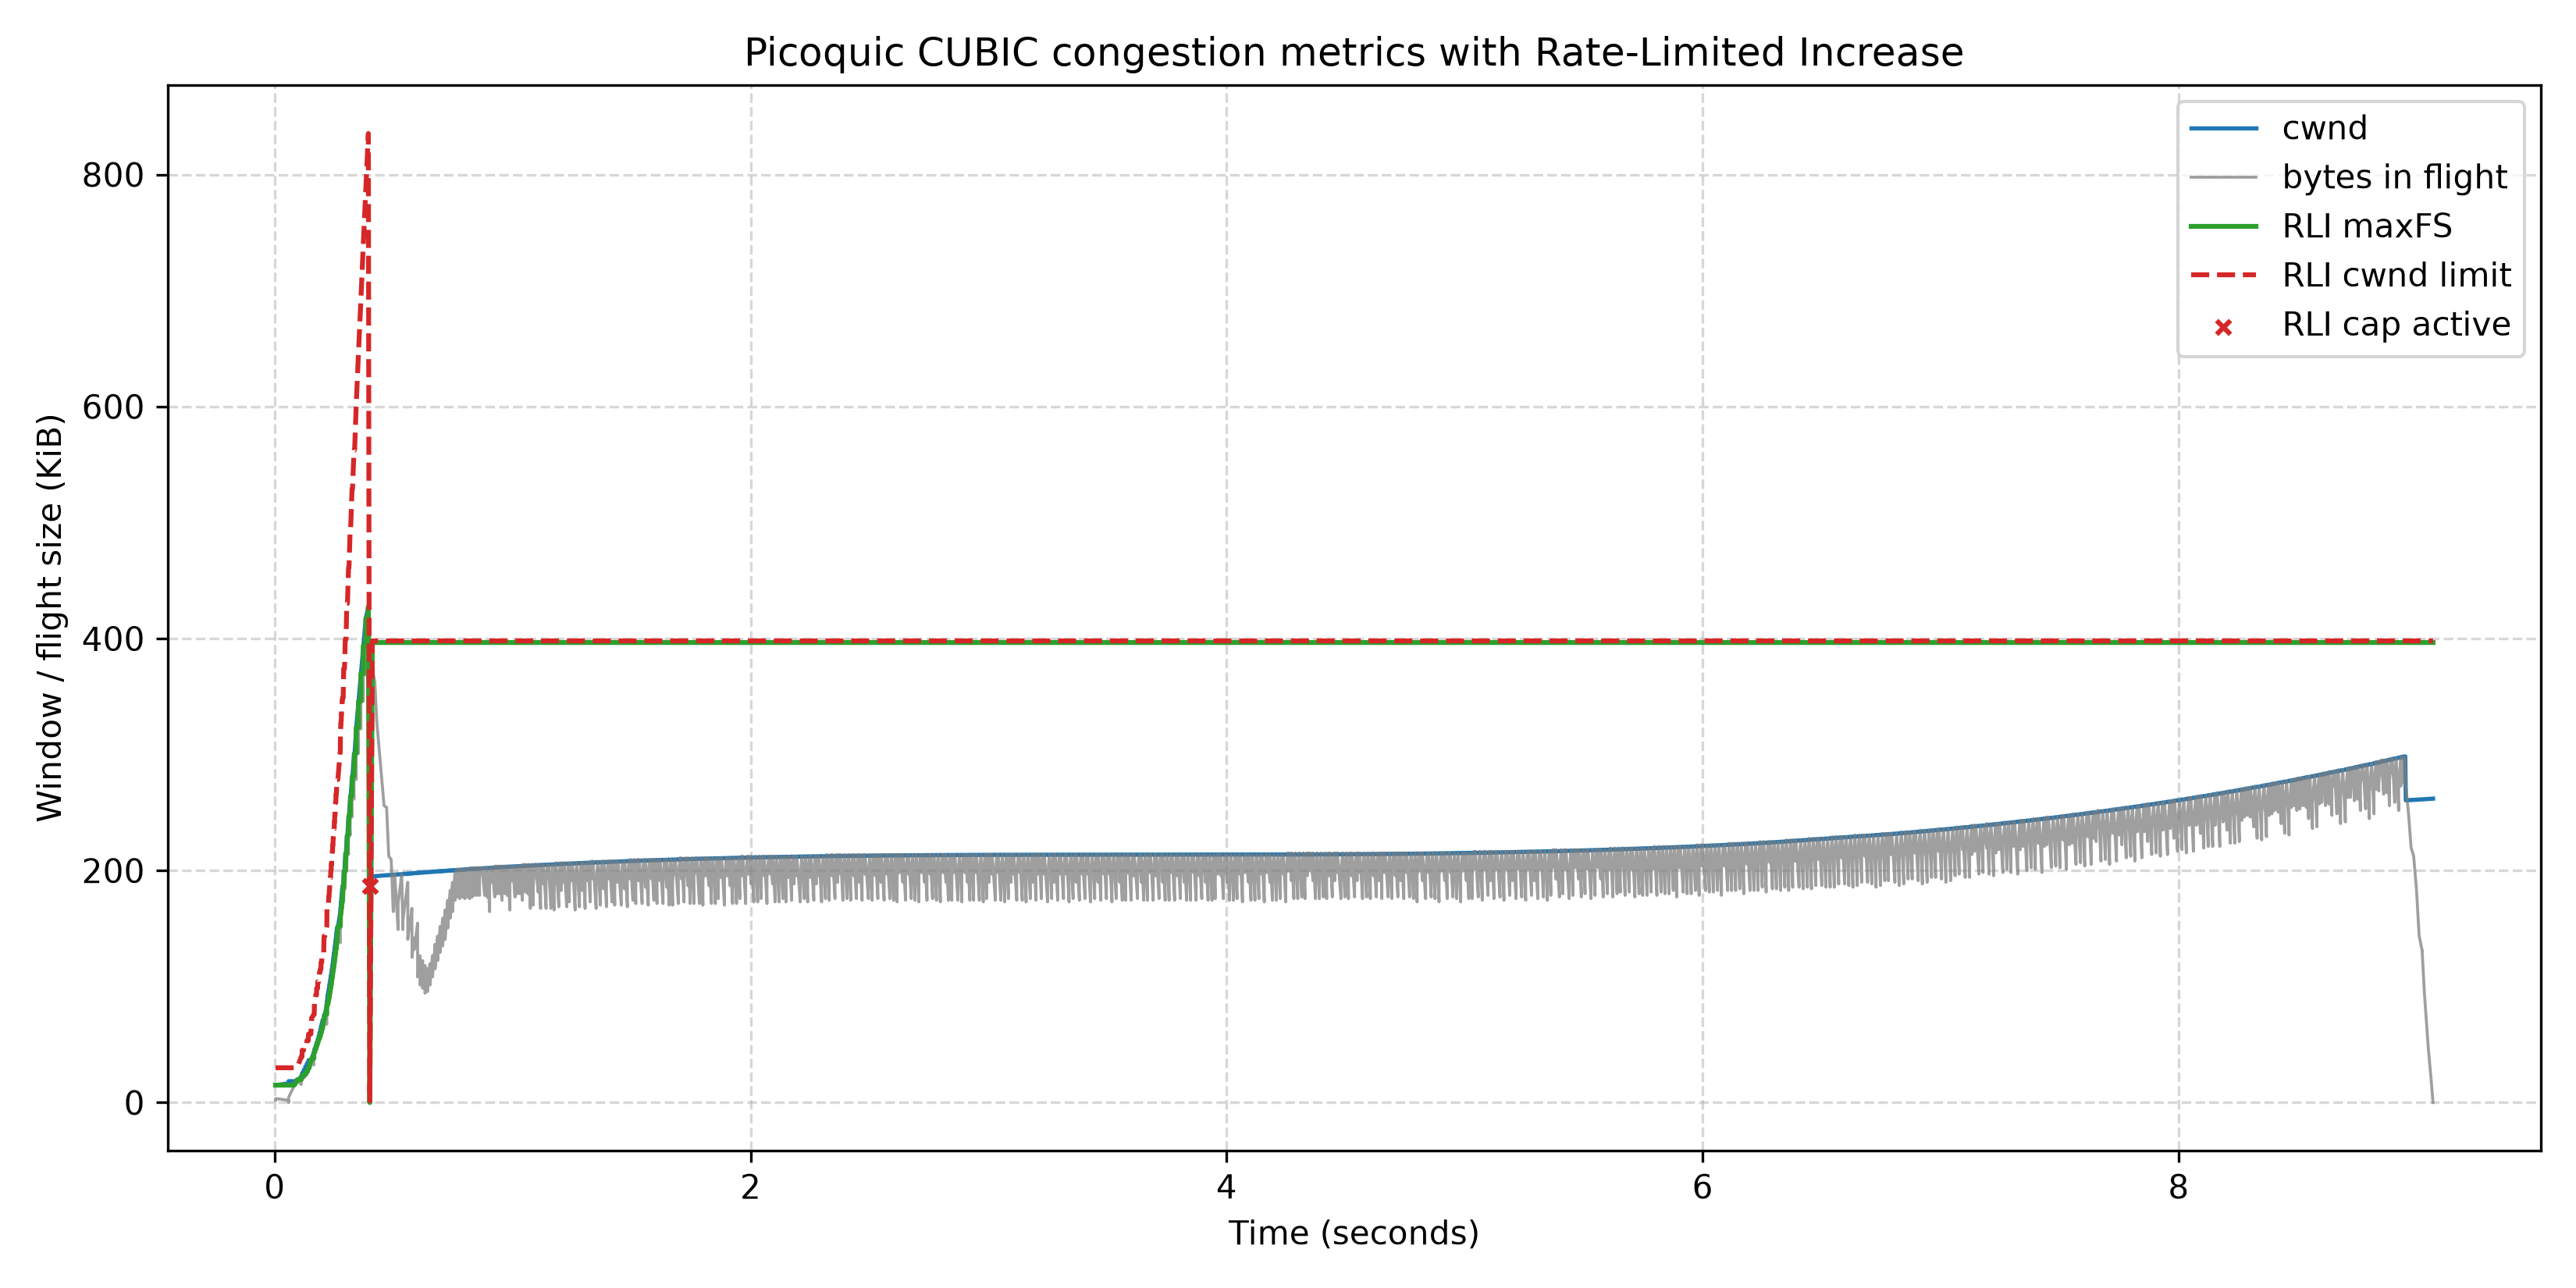
\includegraphics[width=0.92\textwidth]{plots/bulk-rli-2.png}
\caption{Rli: final cwnd 261.98 KiB; time-weighted mean 221.30 KiB; throughput 17.958 Mbit/s.}\end{figure}
These matched traces test a continuously backlogged sender. Normal CUBIC growth and congestion responses dominate; compare measured throughput rather than window height alone.
\clearpage\subsection{Bulk control, repetition 3}
\begin{figure}[H]\centering
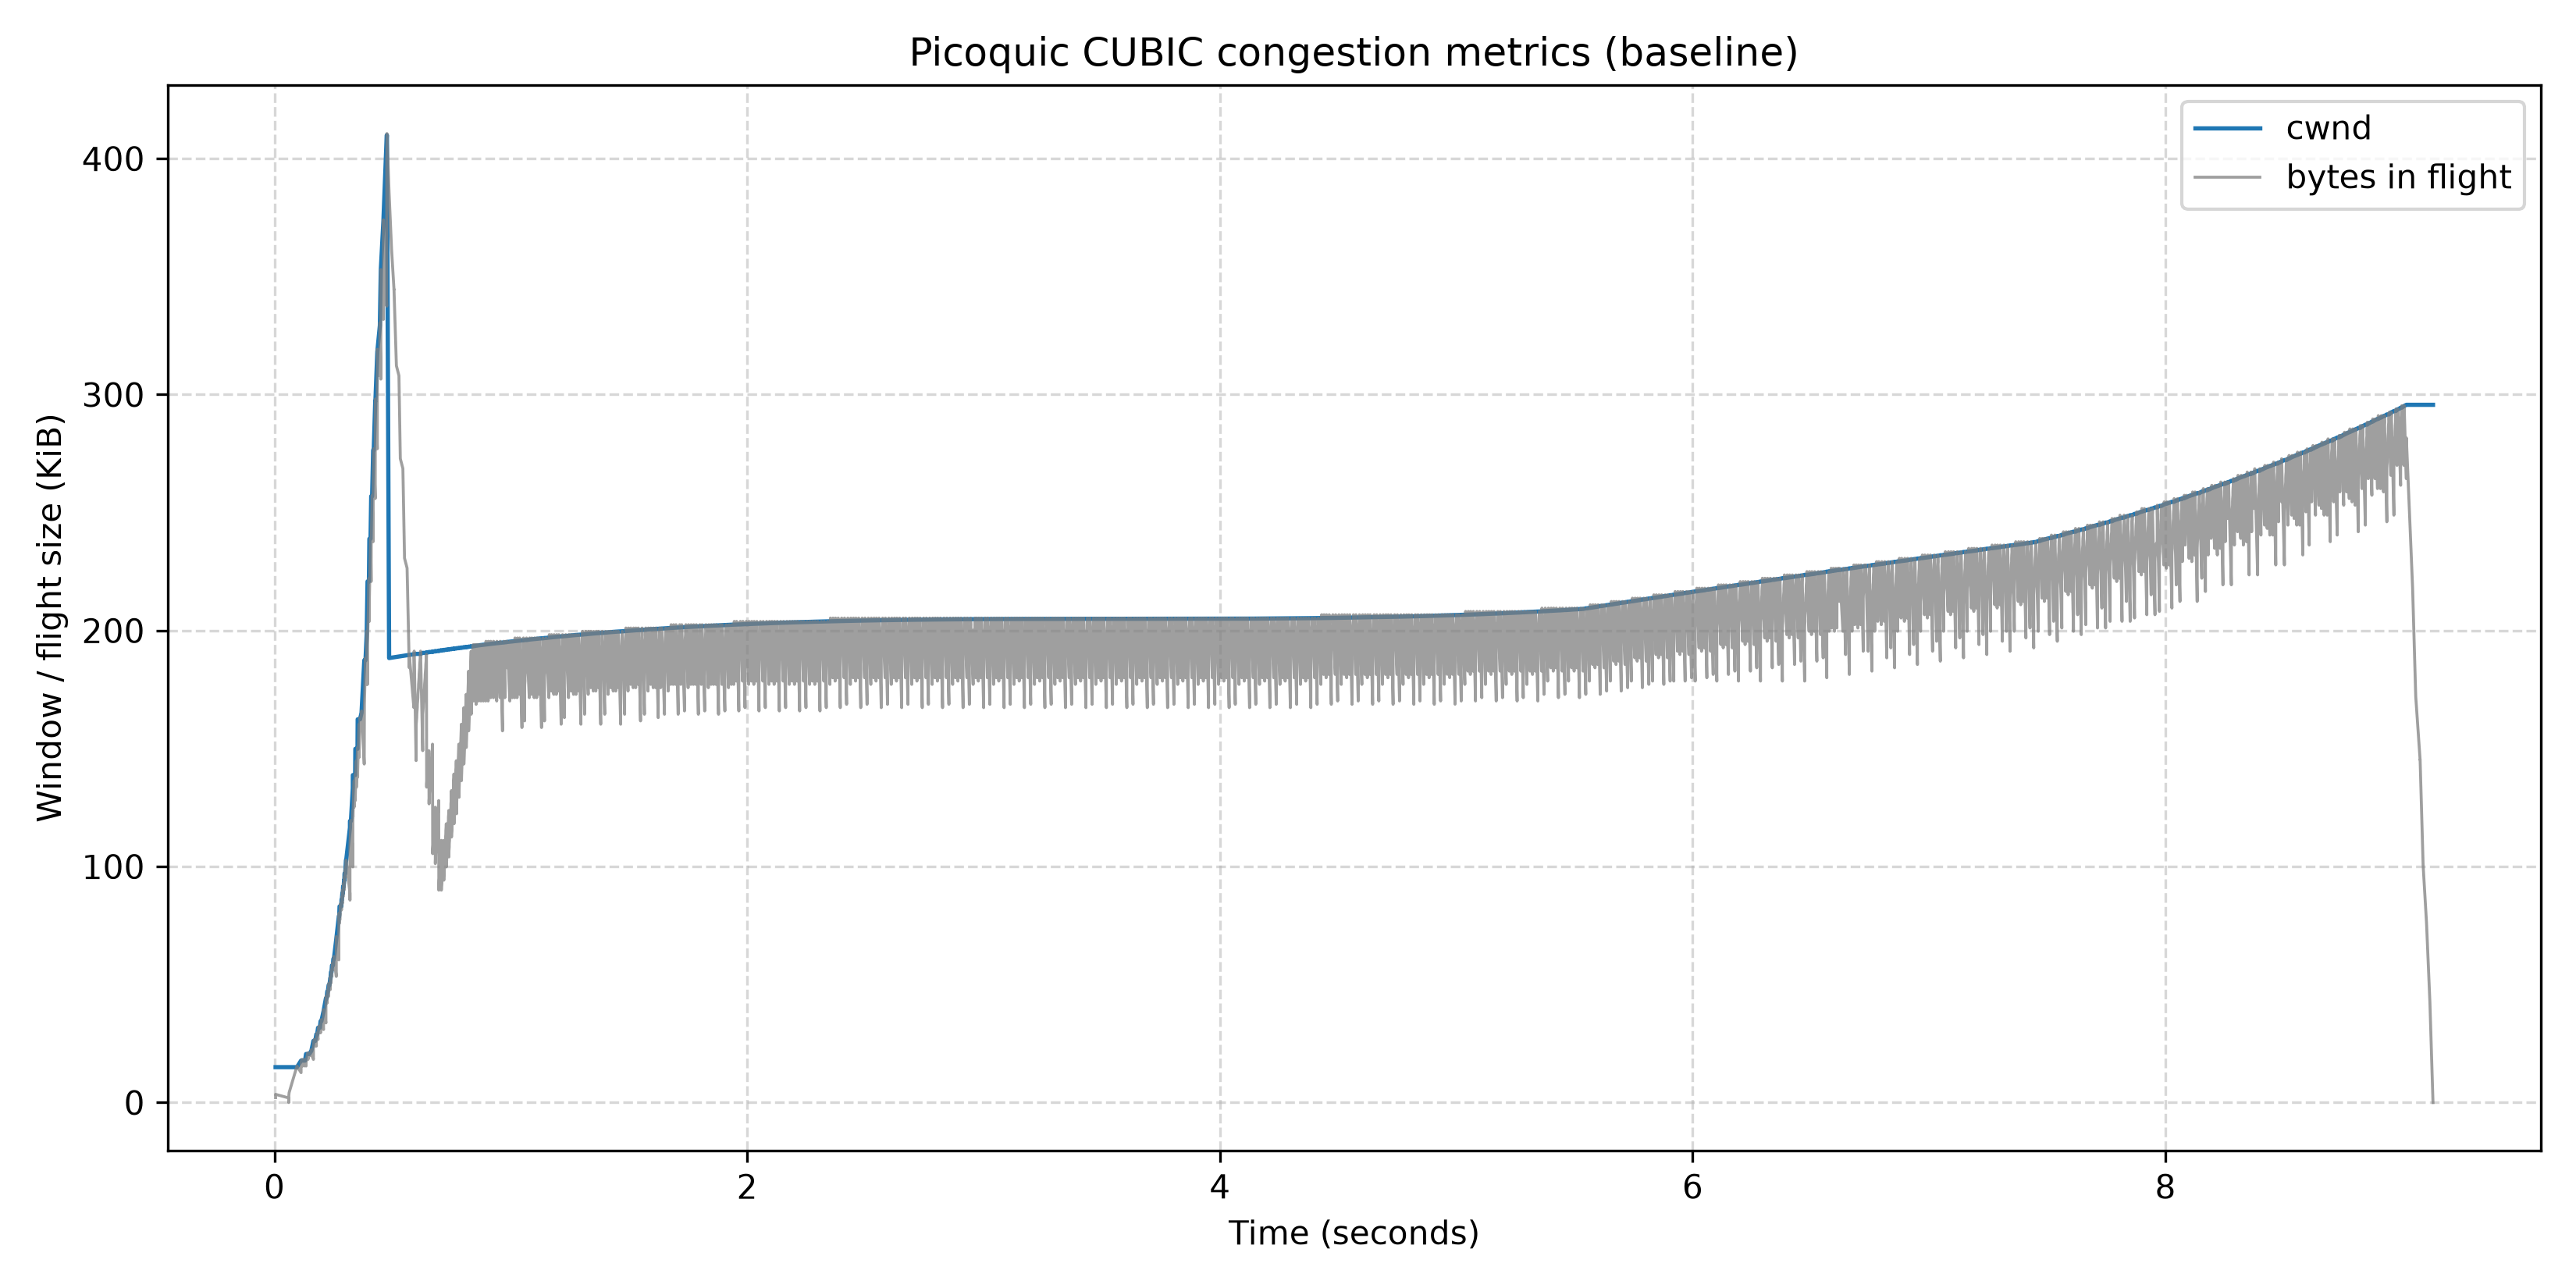
\includegraphics[width=0.92\textwidth]{plots/bulk-baseline-3.png}
\caption{Baseline: final cwnd 295.67 KiB; time-weighted mean 213.74 KiB; throughput 17.640 Mbit/s.}\end{figure}
\begin{figure}[H]\centering
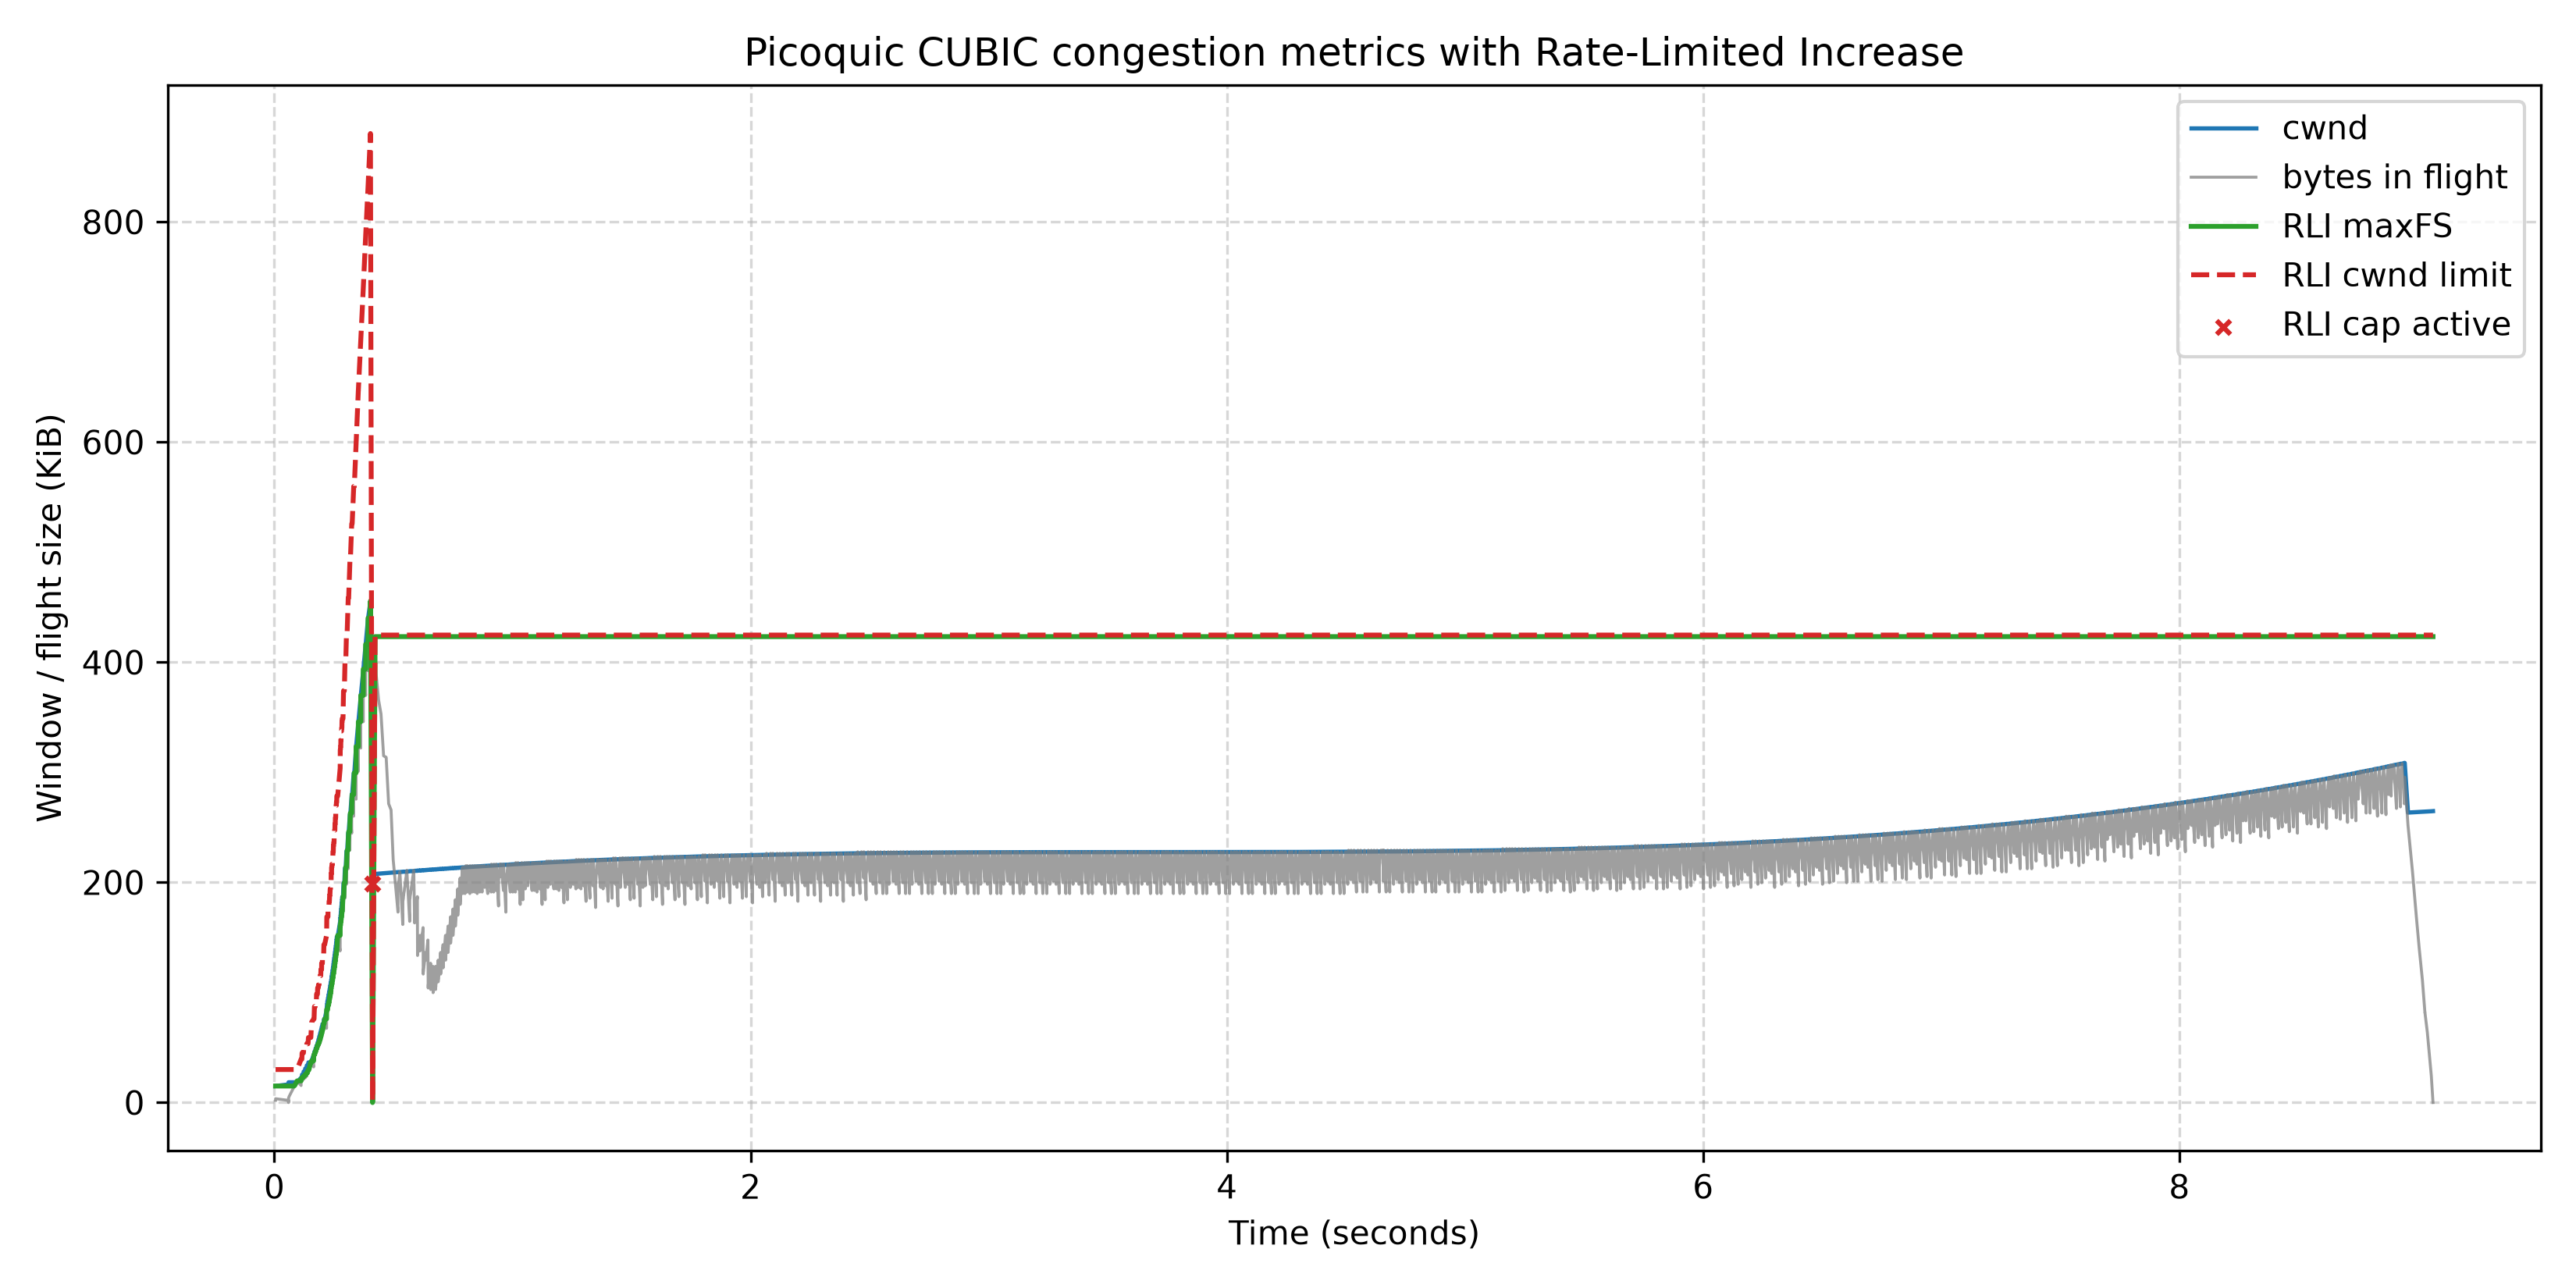
\includegraphics[width=0.92\textwidth]{plots/bulk-rli-3.png}
\caption{Rli: final cwnd 264.75 KiB; time-weighted mean 233.93 KiB; throughput 17.952 Mbit/s.}\end{figure}
These matched traces test a continuously backlogged sender. Normal CUBIC growth and congestion responses dominate; compare measured throughput rather than window height alone.

\clearpage
\section{Competing-flow dumbbell graphs}
Each graph shows two simultaneous 20 MiB transfers over the same bottleneck.
The three matched pairs correspond to the supplementary results table.
\subsection{Two-flow dumbbell, repetition 1}
\begin{figure}[H]\centering
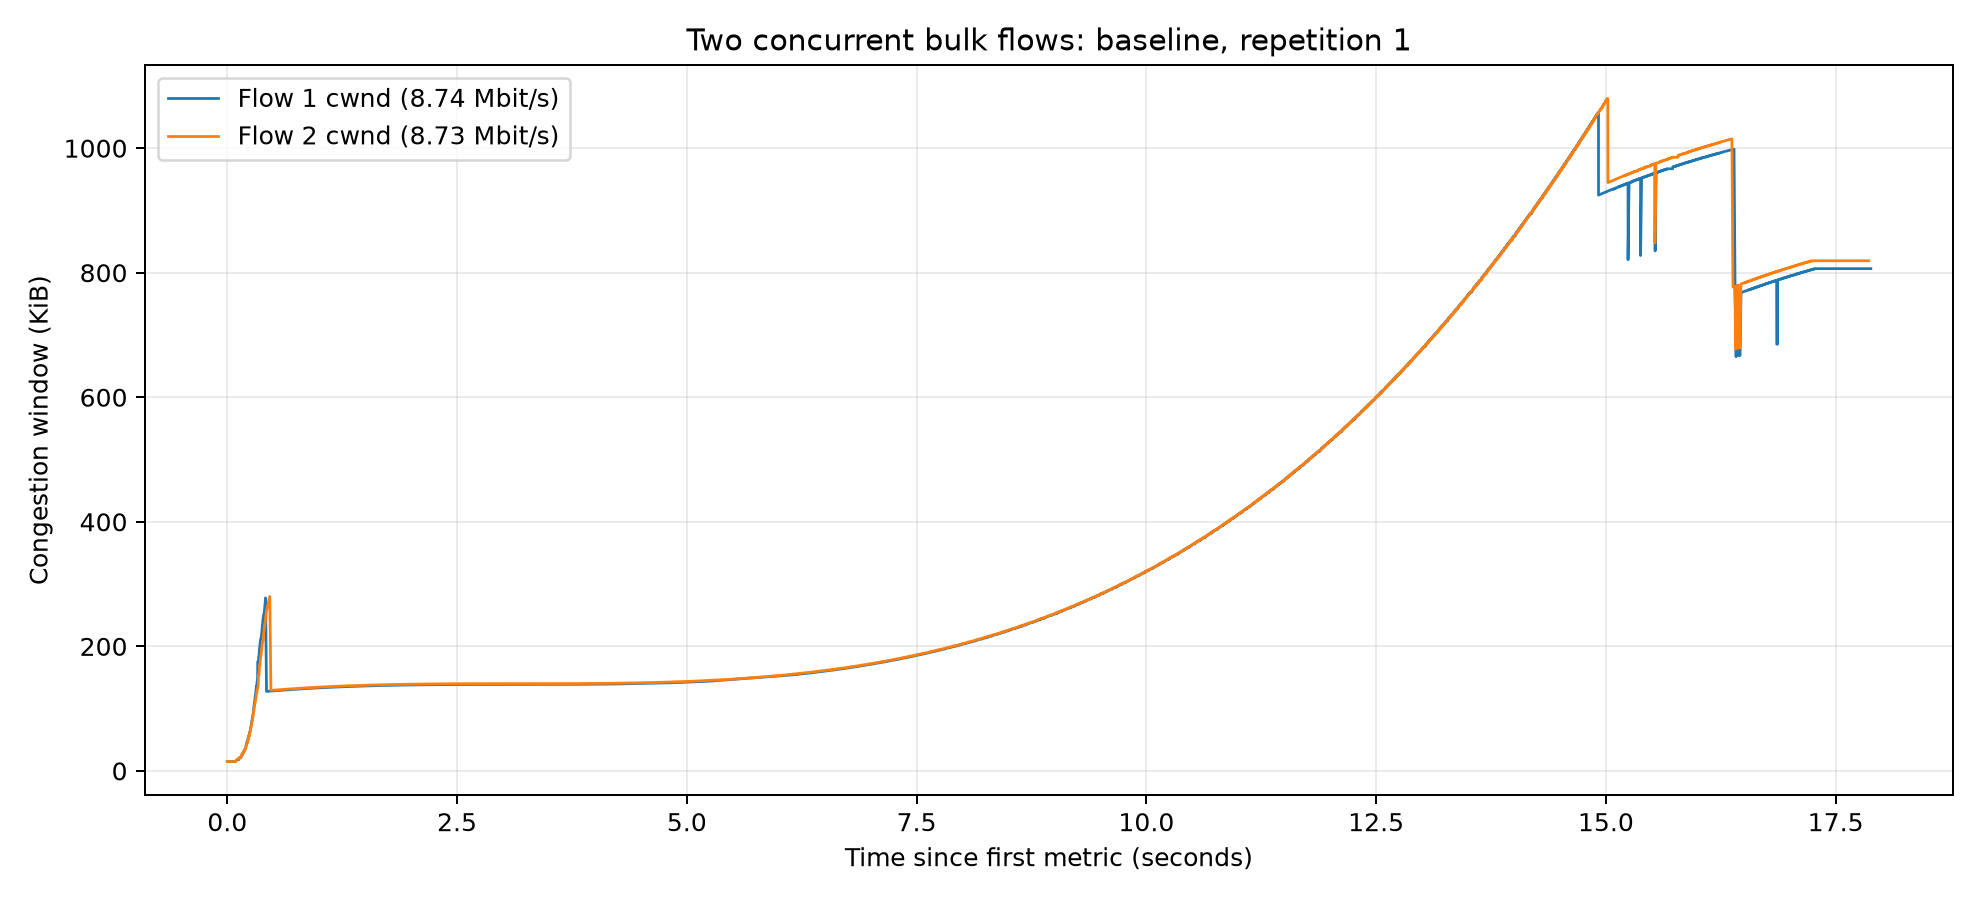
\includegraphics[width=0.92\textwidth]{plots/dumbbell/baseline-1.png}
\caption{Baseline: both client/server pairs transfer 20 MiB concurrently over the shared bottleneck.}\end{figure}
\begin{figure}[H]\centering
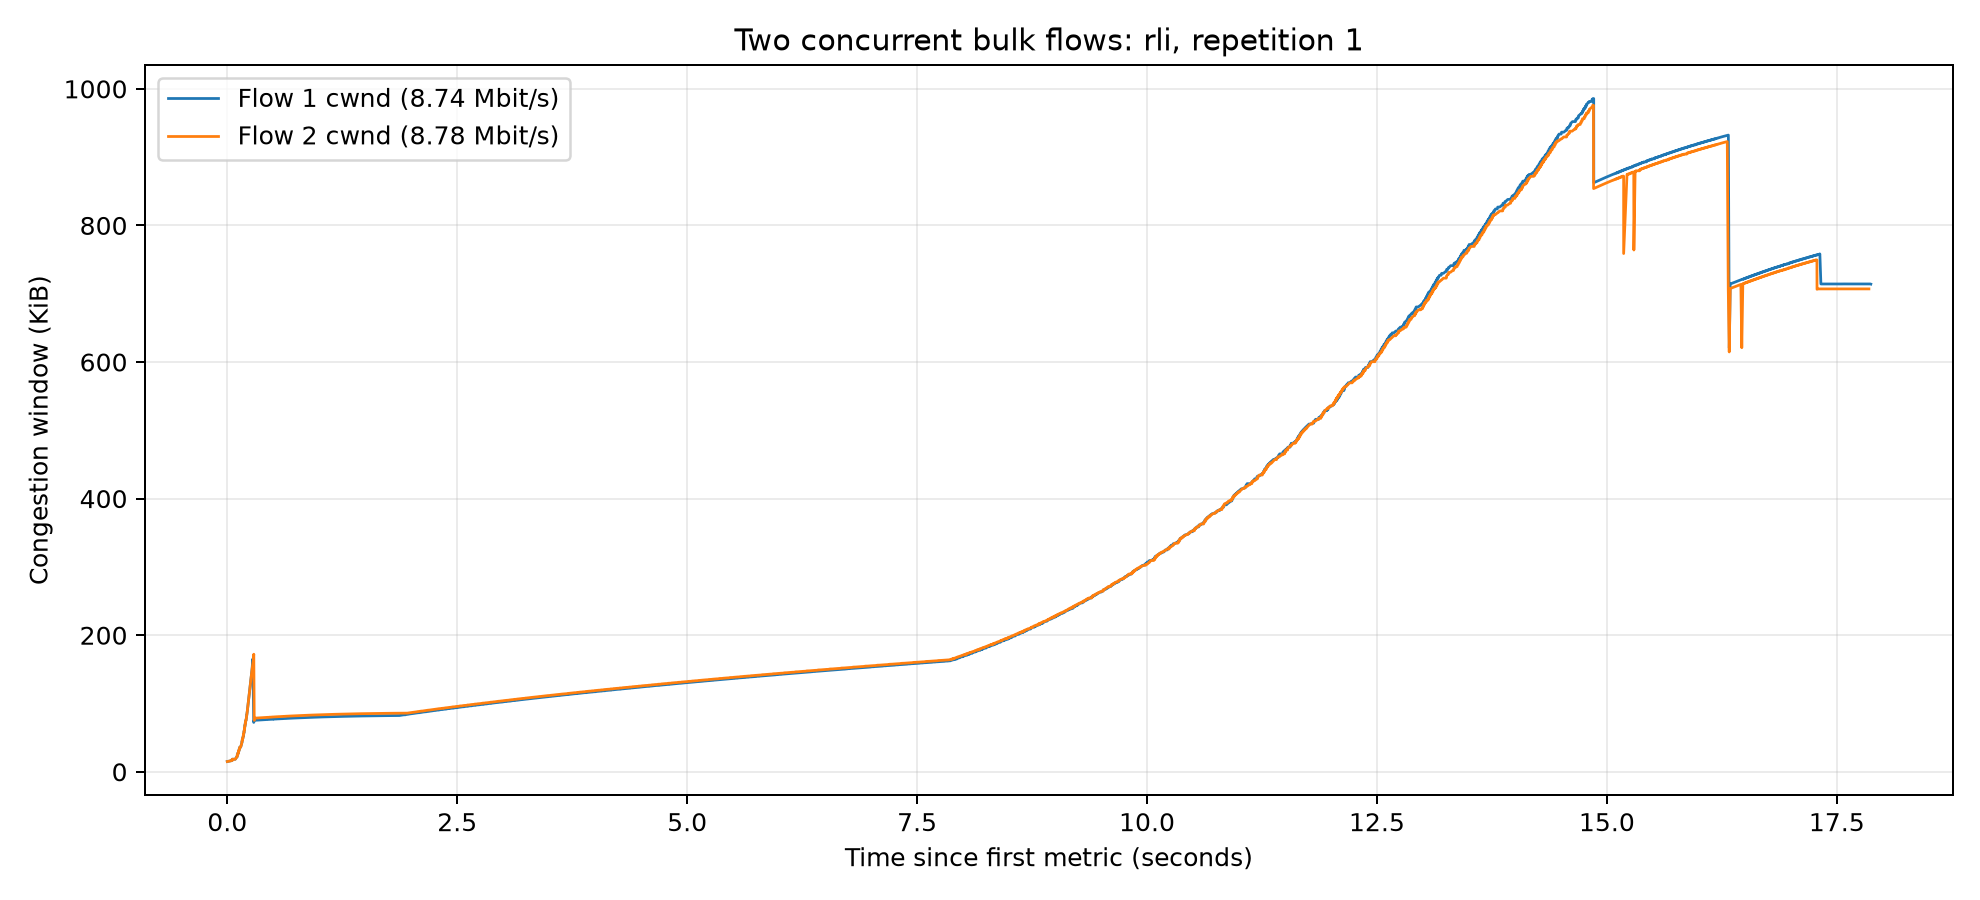
\includegraphics[width=0.92\textwidth]{plots/dumbbell/rli-1.png}
\caption{Rli: both client/server pairs transfer 20 MiB concurrently over the shared bottleneck.}\end{figure}
The two lines show the congestion windows of competing flows. Window height and temporary differences in allocation should be interpreted alongside the transfer rates and Jain index.
\clearpage\subsection{Two-flow dumbbell, repetition 2}
\begin{figure}[H]\centering
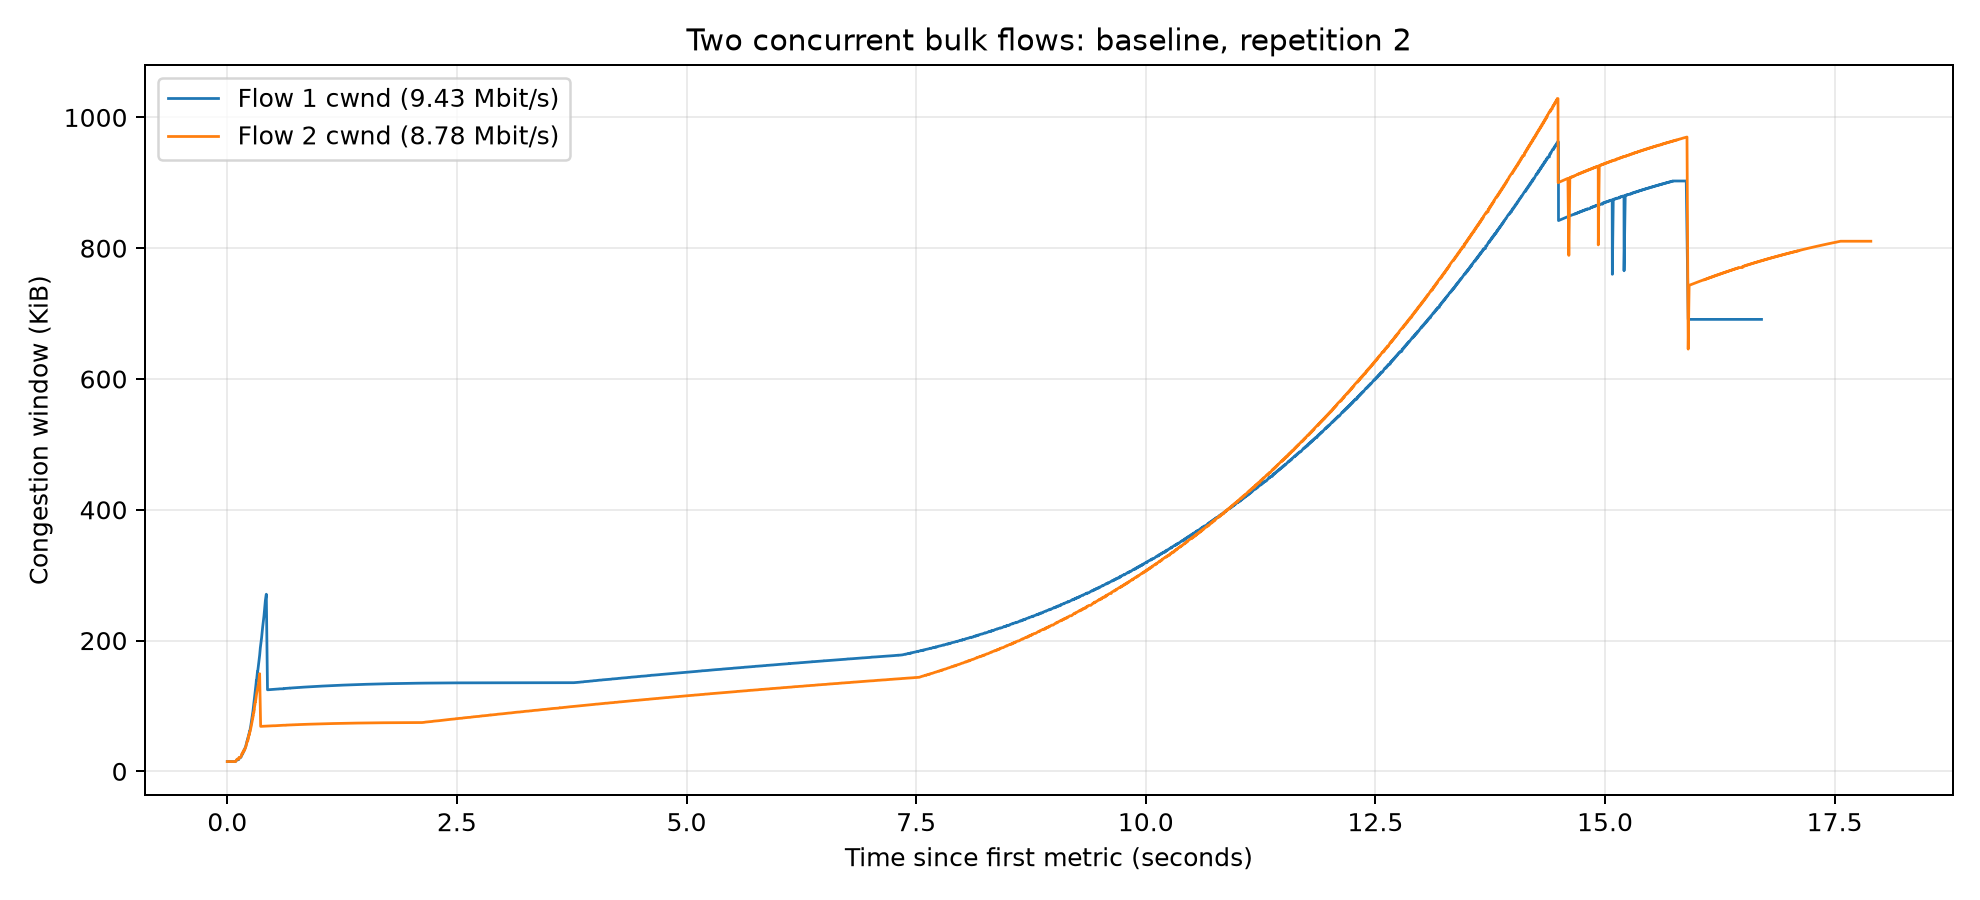
\includegraphics[width=0.92\textwidth]{plots/dumbbell/baseline-2.png}
\caption{Baseline: both client/server pairs transfer 20 MiB concurrently over the shared bottleneck.}\end{figure}
\begin{figure}[H]\centering
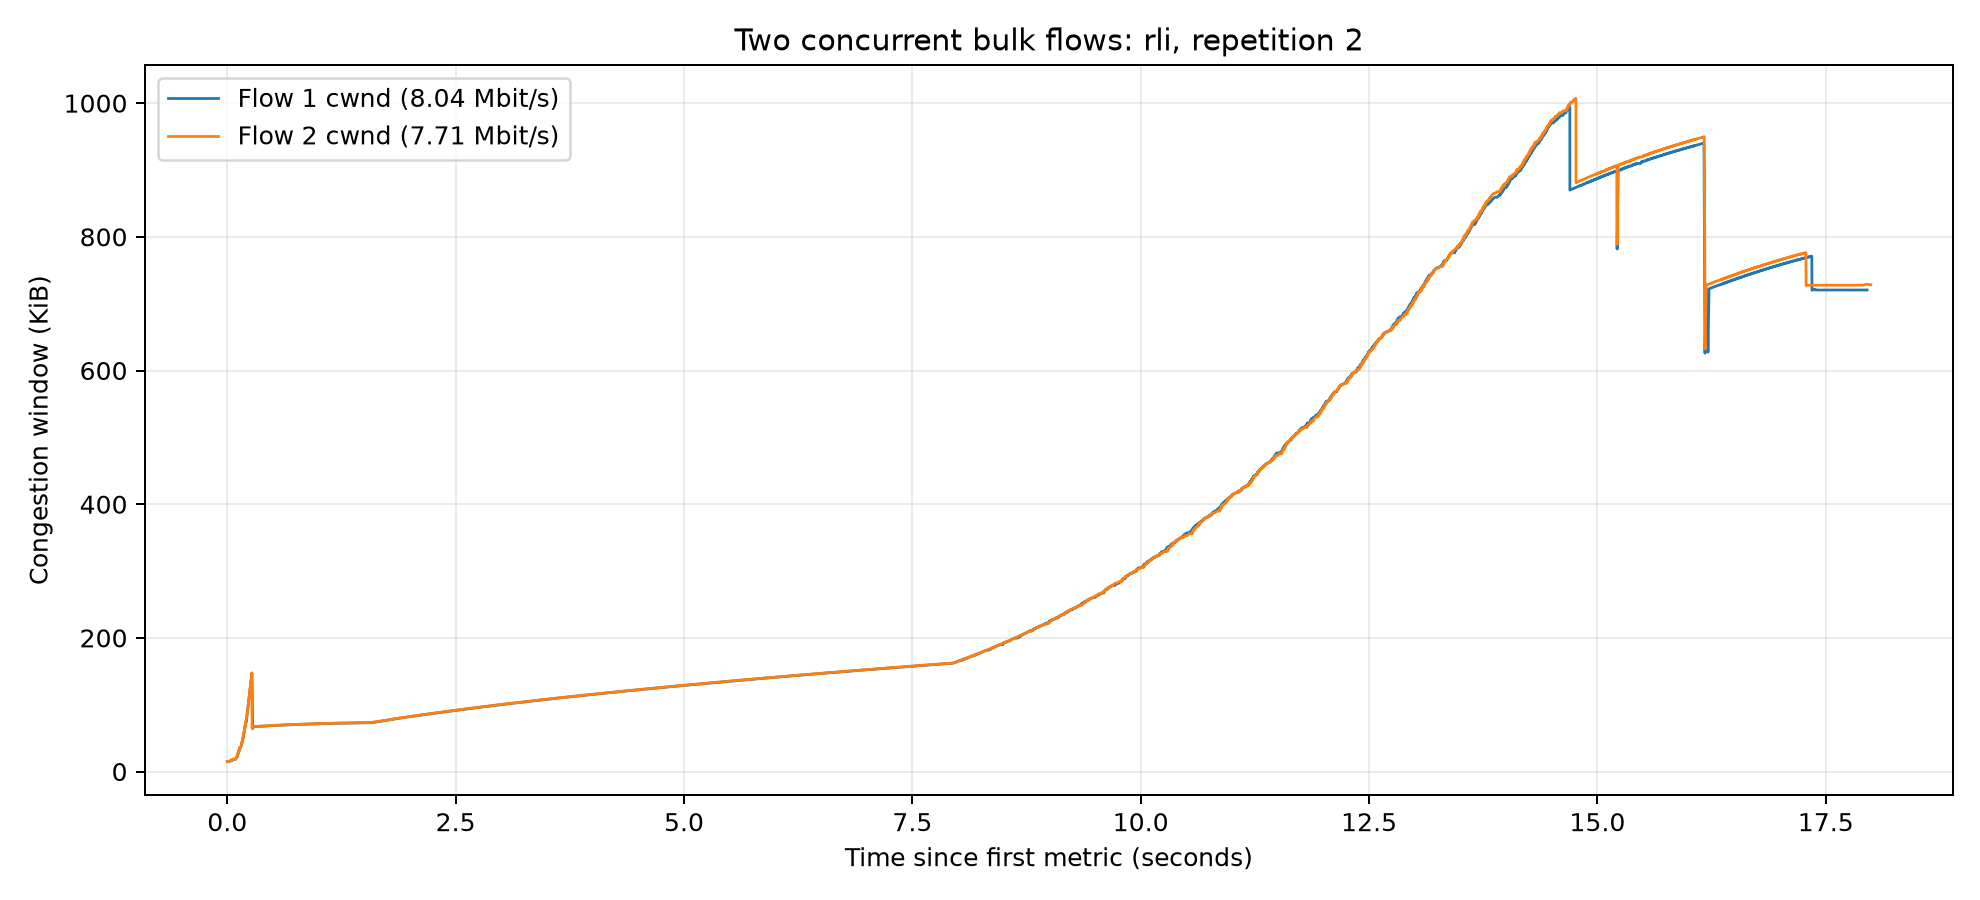
\includegraphics[width=0.92\textwidth]{plots/dumbbell/rli-2.png}
\caption{Rli: both client/server pairs transfer 20 MiB concurrently over the shared bottleneck.}\end{figure}
The two lines show the congestion windows of competing flows. Window height and temporary differences in allocation should be interpreted alongside the transfer rates and Jain index.
\clearpage\subsection{Two-flow dumbbell, repetition 3}
\begin{figure}[H]\centering
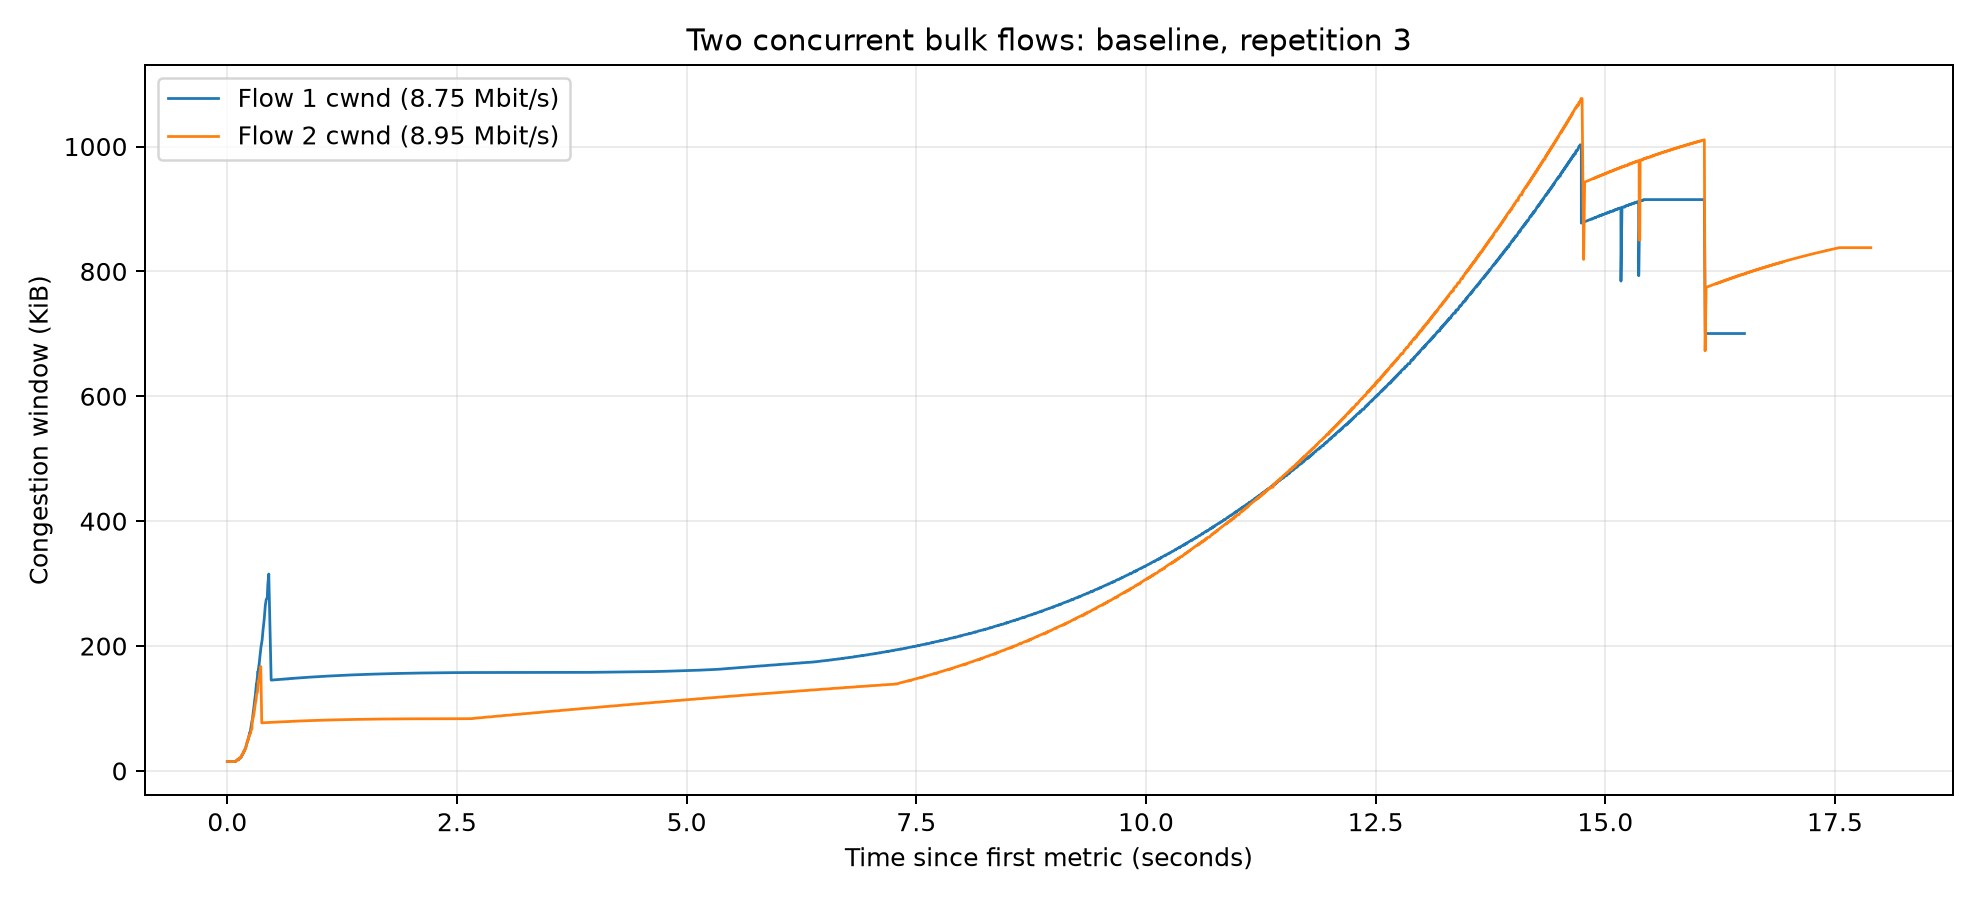
\includegraphics[width=0.92\textwidth]{plots/dumbbell/baseline-3.png}
\caption{Baseline: both client/server pairs transfer 20 MiB concurrently over the shared bottleneck.}\end{figure}
\begin{figure}[H]\centering
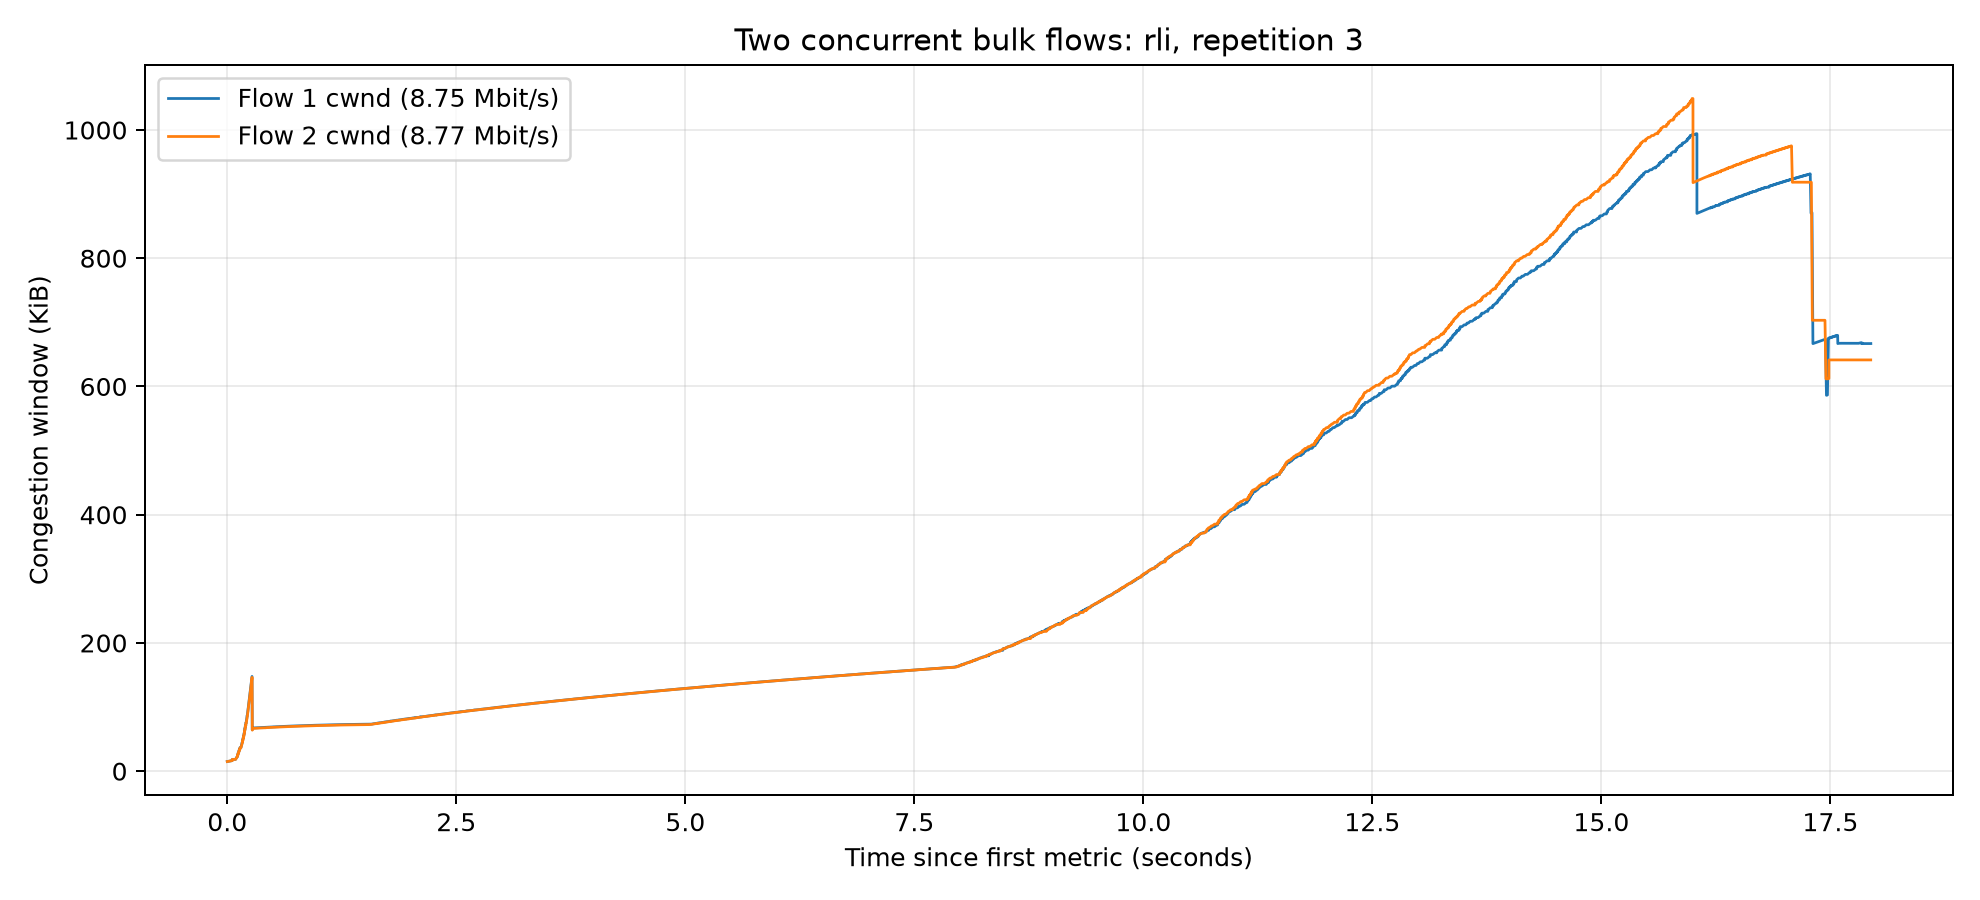
\includegraphics[width=0.92\textwidth]{plots/dumbbell/rli-3.png}
\caption{Rli: both client/server pairs transfer 20 MiB concurrently over the shared bottleneck.}\end{figure}
The two lines show the congestion windows of competing flows. Window height and temporary differences in allocation should be interpreted alongside the transfer rates and Jain index.

\end{document}
